\chapter{Results}
The primary motivation for this research is to learn more about alcoholism, its causes, accompanying characteristics and consequences. In our effort we conducted multiple studies, each taking advantage of a different, uniquely suitable set of tools. We trace their effectiveness, validity and limitations in achieving the thesis objectives of:
\begin{itemize}
	\item describing data in meaningful visual form;
	\item aligning and cross examination of data of different sources;
	\item generating hypothesis;
	\item observing gender and drinking category differences;
	\item understanding the predictive power of the alcohol induction data on the future levels of alcoholism.
\end{itemize}

The chapter describes our major studies and their results, presented in two separate sections. The first section describes five separate investigations aimed at quickly discovering and testing new hypothesis. We found that using Django ORM and Python's SciPy ecosystem greatly facilitates that task. Using various analytical tools, described in detail below, we demonstrate the following findings: 
\begin{itemize}
	\item Animals increase their need for fluid after they eat. Heavy drinking animals appear to have a preference of alcohol over the water resulting in peaks in alcohol consumption after the food intake. 
	\item Drink-to-bout ratio is a good indicator of habitual drinking. KDE plot reveals a divergence of habitual drinking between females when the periods of first nine months versus last three months are considered. This is not the case for males.
	\item Menstrual cycle strongly affects alcohol consumption in females. Peaks in ethanol drinking follows the peaks of progesterone levels with the lag of few days. Females appear to drink more alcohol in their post-luni phase of the menstrual cycle.
	\item Binge drinking animal have a sporadic drinking pattern. Low and binge drinkers are averse of drinking on the day after intoxication. On contrast, heavy drinkers appear to tolerate intoxication well, which, on the other hand, may indicate the innate inability to quit drinking. 
	\item Heavy drinking females reduce their alcohol consumption much less the day
	after intoxication than low drinking ones; conversely, heavy drinking males reduce
	their drinking more the day after intoxication than low drinking ones.
\end{itemize}

The second section describes the detailed study of the prediction of future levels of alcoholism based on the early (induction) drinking and behavioral data using machine learning techniques. Our main contributions are in creating new attributes, generating relative feature reflective of adaptation process, adjusting Random Forests model and developing novel two-step classification model. 

\section{Discovering and Testing New Hypothesis}
	Given the large volumes of data describing each sample, it is desirable to produce new hypothesis with regard of the general population. Slicing and aggregating data by new angles and visualizing it gives us opportunity to identify anomalies or tendencies and make a hypothesis. Additionally, employees that work with the animals directly notice peculiarities in the animal behavior, which may lead to apriori knowledge. A biologist can infer what the causes of that might be, and a data analyst can test hypothesis given the appropriate data is present. 	
	
\pagebreak	
	\subsection{Drinking Pattern}
	Recall that during the open access phase of the experiment, concurrent access to water and alcohol solution is available to the subjects. Each day's session lasts 22 hours, which guarantees at least two hours of no alcohol for heavy drinkers. At the end of the eighth hour of the session the lights in the cages are turned off; at the beginning of the 20th hour the lights are turned on. Food pellets are available on demand in specified intervals during the day, starting at hour zero. 
	
	One objective is to determine whether or not the drinking patterns of low drinkers differ significantly from that of heavy drinkers. To answer this question we needed a visual representation of alcohol consumption during the day by each animal. The problem is that the drinking varies from day to day, and we need to see ``averaged" picture. 
	
	In the database we store raw data about alcohol drinks (defined as drinking without stop for more than five seconds) during the day by each subject. Each drink is a row with the values for drink start time, drink stop time and the amount consumed. To produce the ``average" drinking pattern for each animal we retrieve the data about the drinks and current weight, and then apply the algorithm~\ref{alg:cum-drink-pattern}:
	
	\begin{algorithm}[H]	%TODO better package for algorithm	
		%\KwData{this text}
		%\KwResult{how to write algorithm with \LaTeX2e }
		%initialization\;
		1. \ForEach{Session}{
			1.1. Get the list of drink as tuples (volume, end time)\; 
			1.2. Replace each tuple's volume with EtOH (g/kg) = volume / animal.weight\;
			1.3. Sort the list by ``end time"\;
		}
		2. Merge each session's list of tuples into one long list\;
		3. Sort the list by ``end time"\;
		4. Apply cumulative sum operation on the EtOH (g/kg) in the list\;
		5. Divide all EtOH (g/kg) by the total number of sessions.
	\caption{Calculating cumulative average drinking pattern.}
	\label{alg:cum-drink-pattern}
	\end{algorithm}
	
	\begin{figure}[ht]
		\centering
		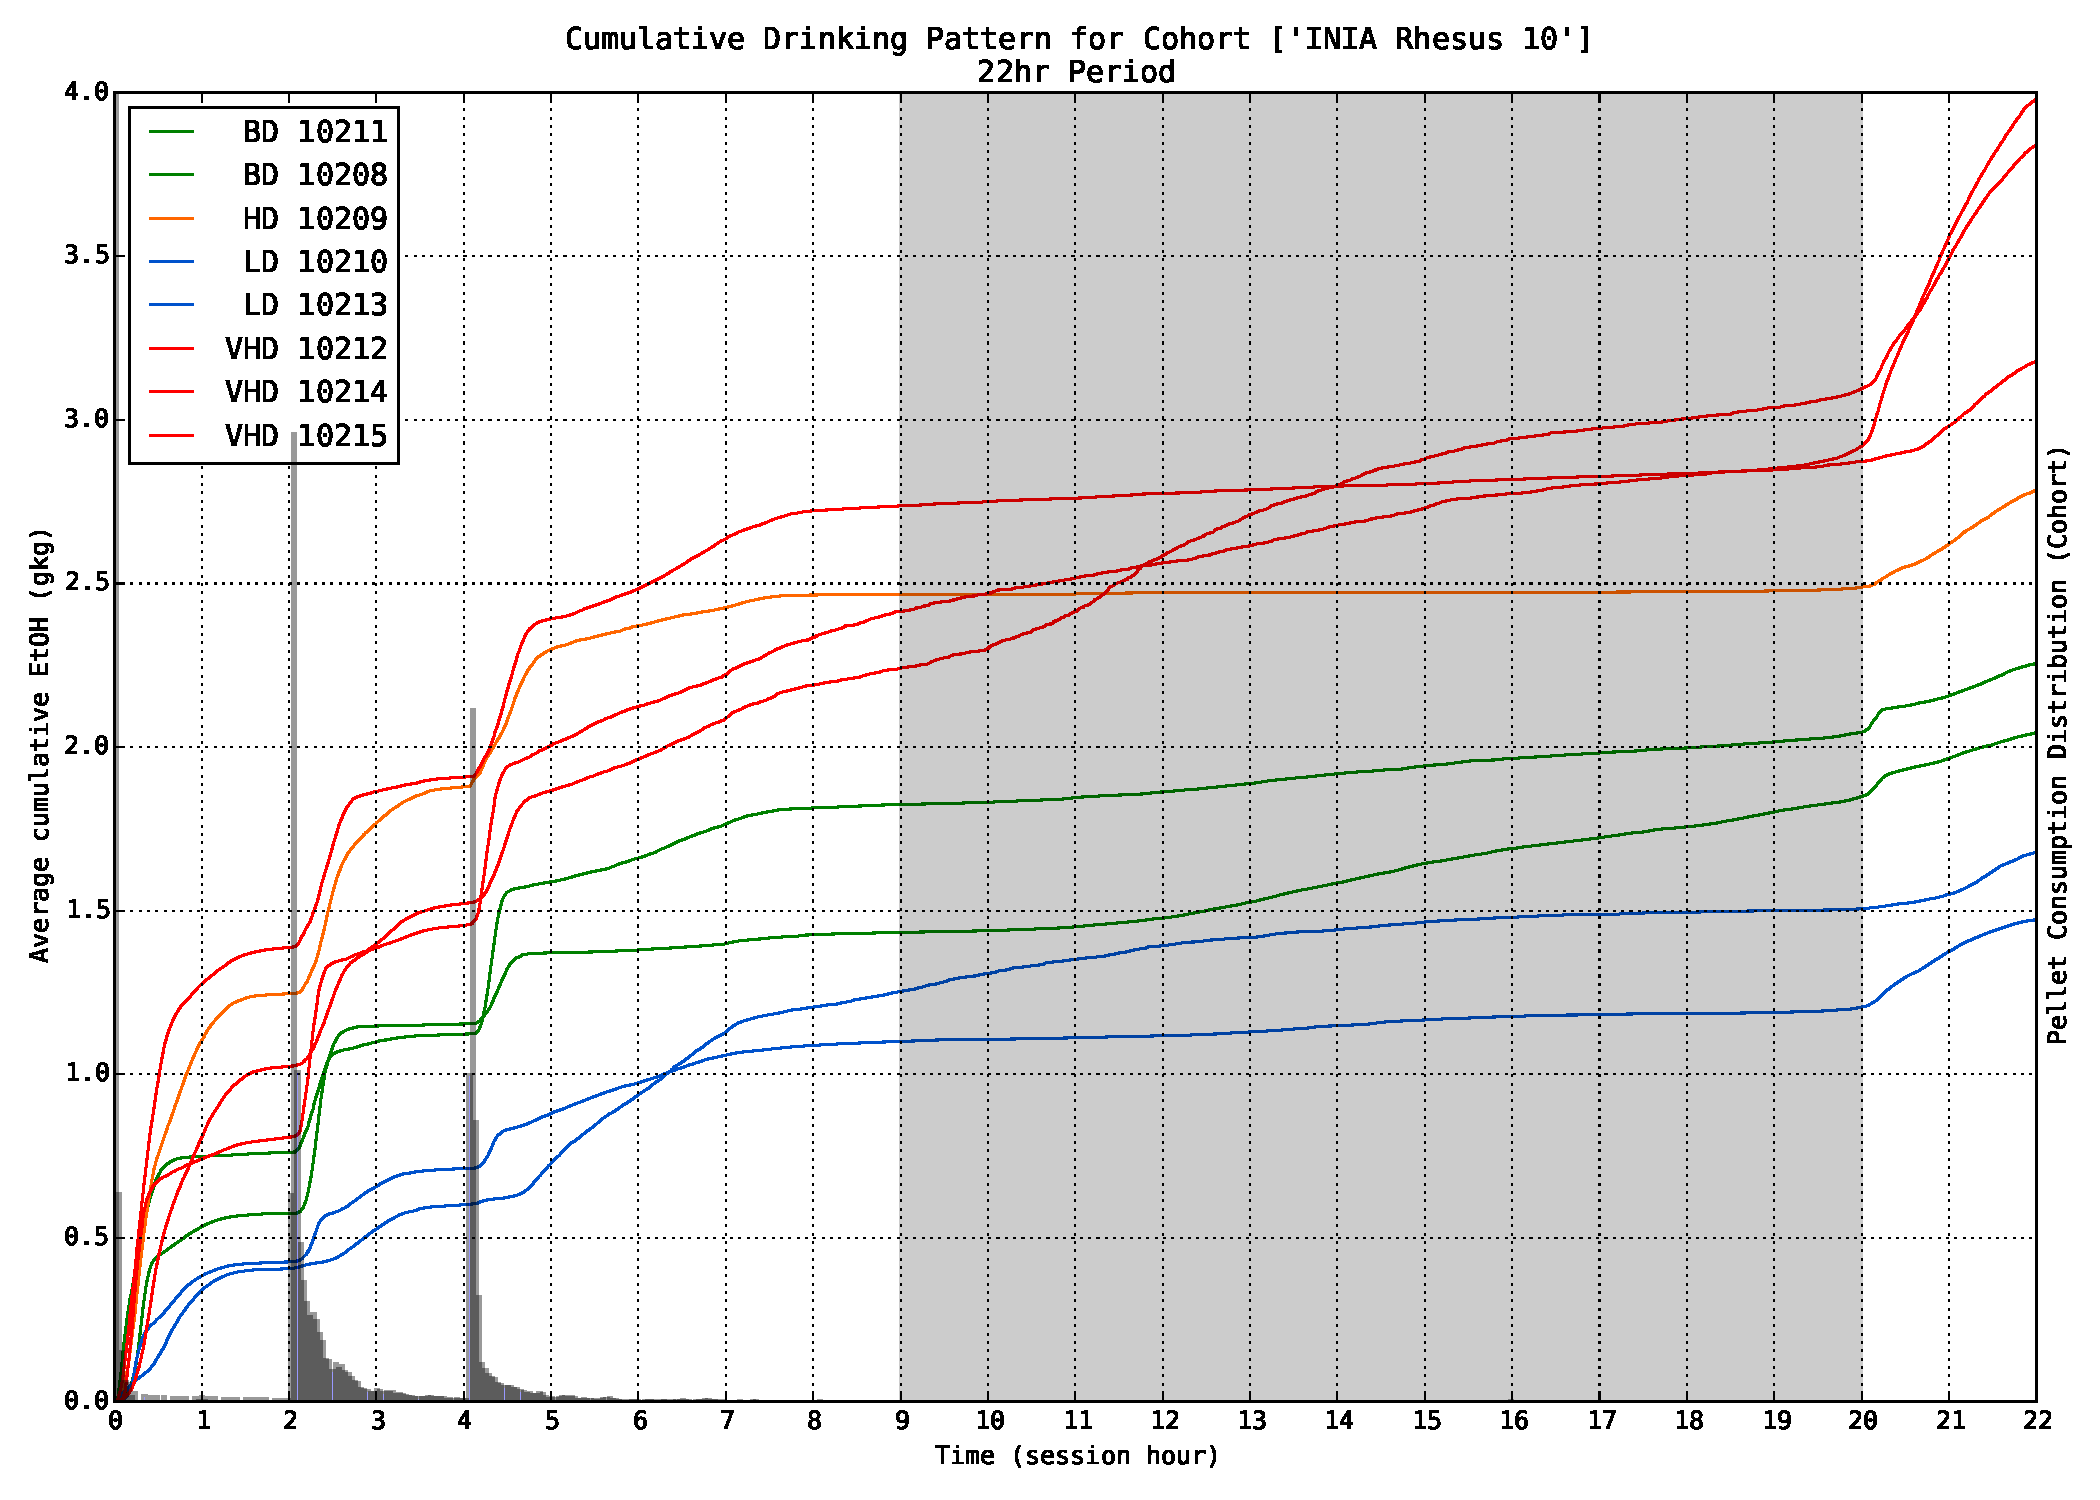
\includegraphics[width=\linewidth]{figures/dp_r10_m_22hr.pdf}
		\caption{Cumulative average drinking pattern plot for 22 hour session. Dark area depicts when lights were off in the cage. Lines show ethanol consumption for each animal. Histogram illustrates food pellet time distribution for the entire cohort.}
		\label{fig:dp-22hr}
	\end{figure}
		
	Algorithm~\ref{alg:cum-drink-pattern} produces normalized cumulative average drinking patter for each animal. The visual representation of the output of the algorithm for cohort ``INIA Rhesus 10" is shown in Figure~\ref{fig:dp-22hr}. The picture has peculiar distinct ``steps" in the lines of cumulative alcohol consumption. In an attempt to explain such phenomena we added food pellet distribution for the entire cohort in form of the histogram. Notably, while drinking patterns do not seem to be different for animals of different drinking category, food consumption has strong influence on alcohol consumption. This may be attributed to the fact that animals typically need fluid after they eat, regardless of what fluid might be. Low drinking animals may prefer water while heavy drinkers prefer the solution of 
	%sugary 
	water with alcohol. Overall, however, all animals drink more alcohol after they eat. 
	
	Another idea for improvement came from the lab employees. They noticed that animals started to drink alcohol as soon as staff appeared in the lab and before the lights actually turned on. Thus we decided to combine the data from the last two hours of the previous day with the current day. We noticed that there is not much activity during the lights off phase, thus used only first nine hours of the current day. Additionally, we de-trended each line of alcohol consumption by subtracting values of the linear regression line, individually for each animal. The result, for cohort ``INIA Rhesus 6b" is presented on Figure~\ref{fig:dp-dl}. Notably, low drinkers have much flatter lines then heavy drinkers who boost their alcohol consumption after the food pellet intake. The early noise does not appear to correlate with drinking behavior, however. 
	
	\begin{figure}[ht]		
		\centering
		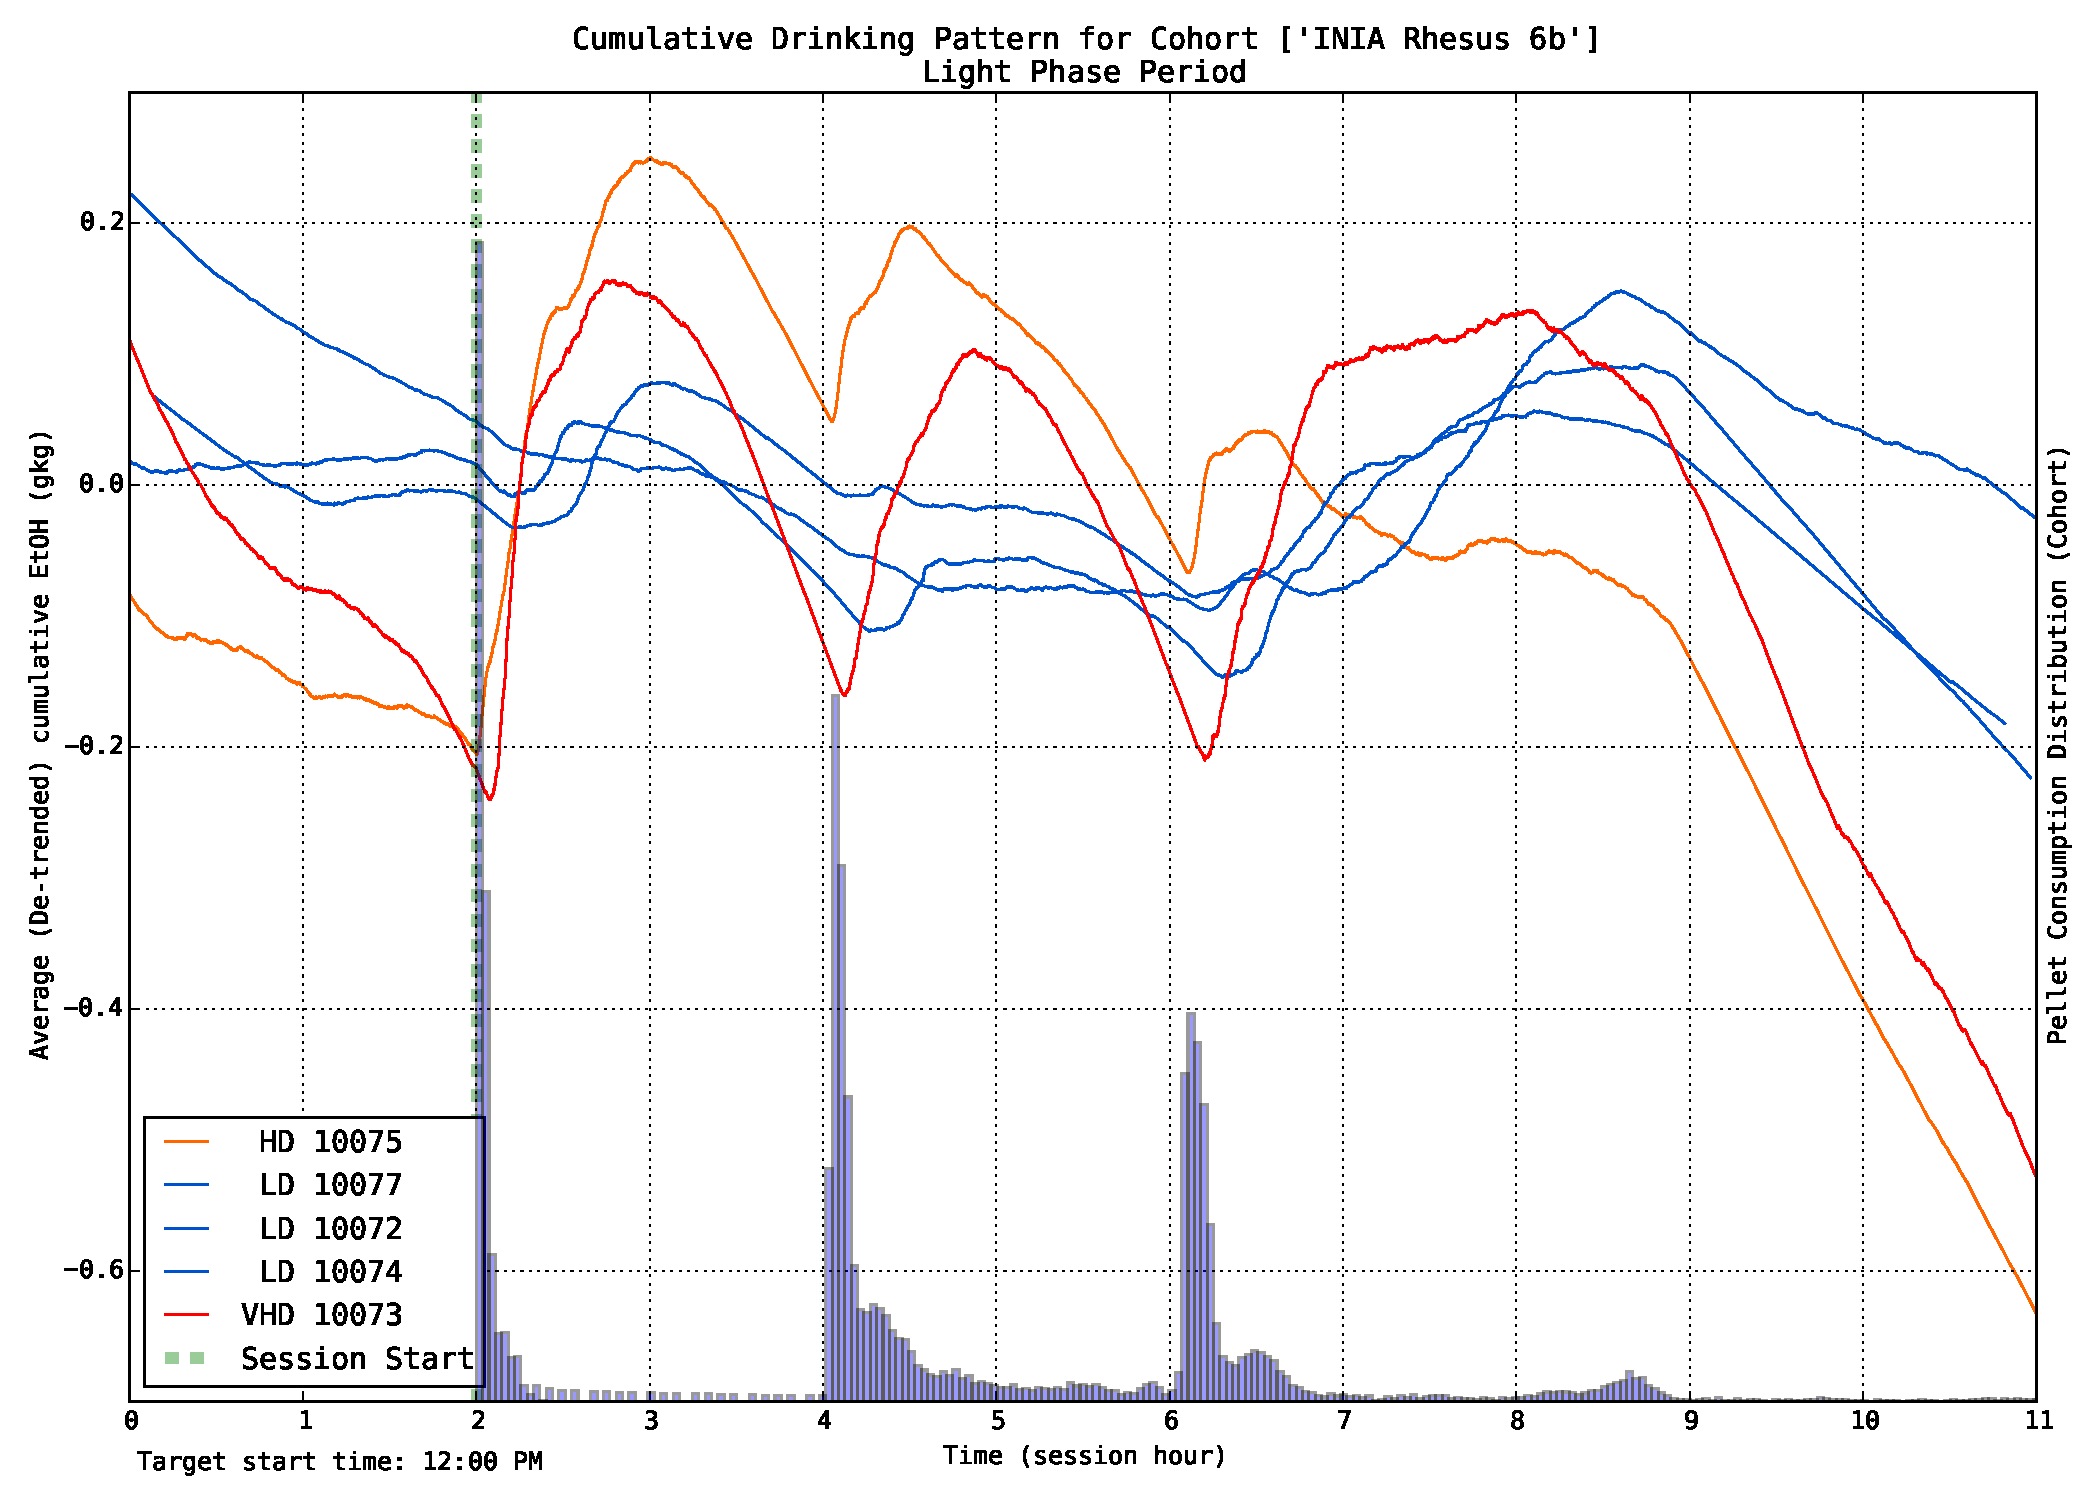
\includegraphics[width=0.98\linewidth]{figures/dp_r6b_f_lights.pdf}
		\caption{Cumulative (de-trended) average drinking pattern plot for daylight session, which includes two hours of the previous day plus nine hours of the current day. Lines illustrate (de-trended) ethanol consumption for each animal. Trend was calculated individually for each animal via linear regression of the first order. Histogram shows food pellet time distribution for the entire cohort.}
		\label{fig:dp-dl}
	\end{figure}
	
		
	\subsection{Habitual Drinking}
	The motivation for the habitual drinking study is to see if there are the differences between males and females in how their drinking habits change from the first nine months to the last three months of the open access. To capture \textit{habitual} drinking we observe the relationship between the mean drink length and the mean bout length. Thus a new daily attribute \textit{``drink-bout ratio"} is created. Factor boxplots can be used to compare between genders, drinking categories and time period, as shown in Figure~\ref{fig:habitual-boxplots-mf}. Such boxplots were created for each available attribute and for each drinking category. Looking through such boxplots allows us to generate new hypothesis.
	
	\begin{figure}[ht]
		\centering
		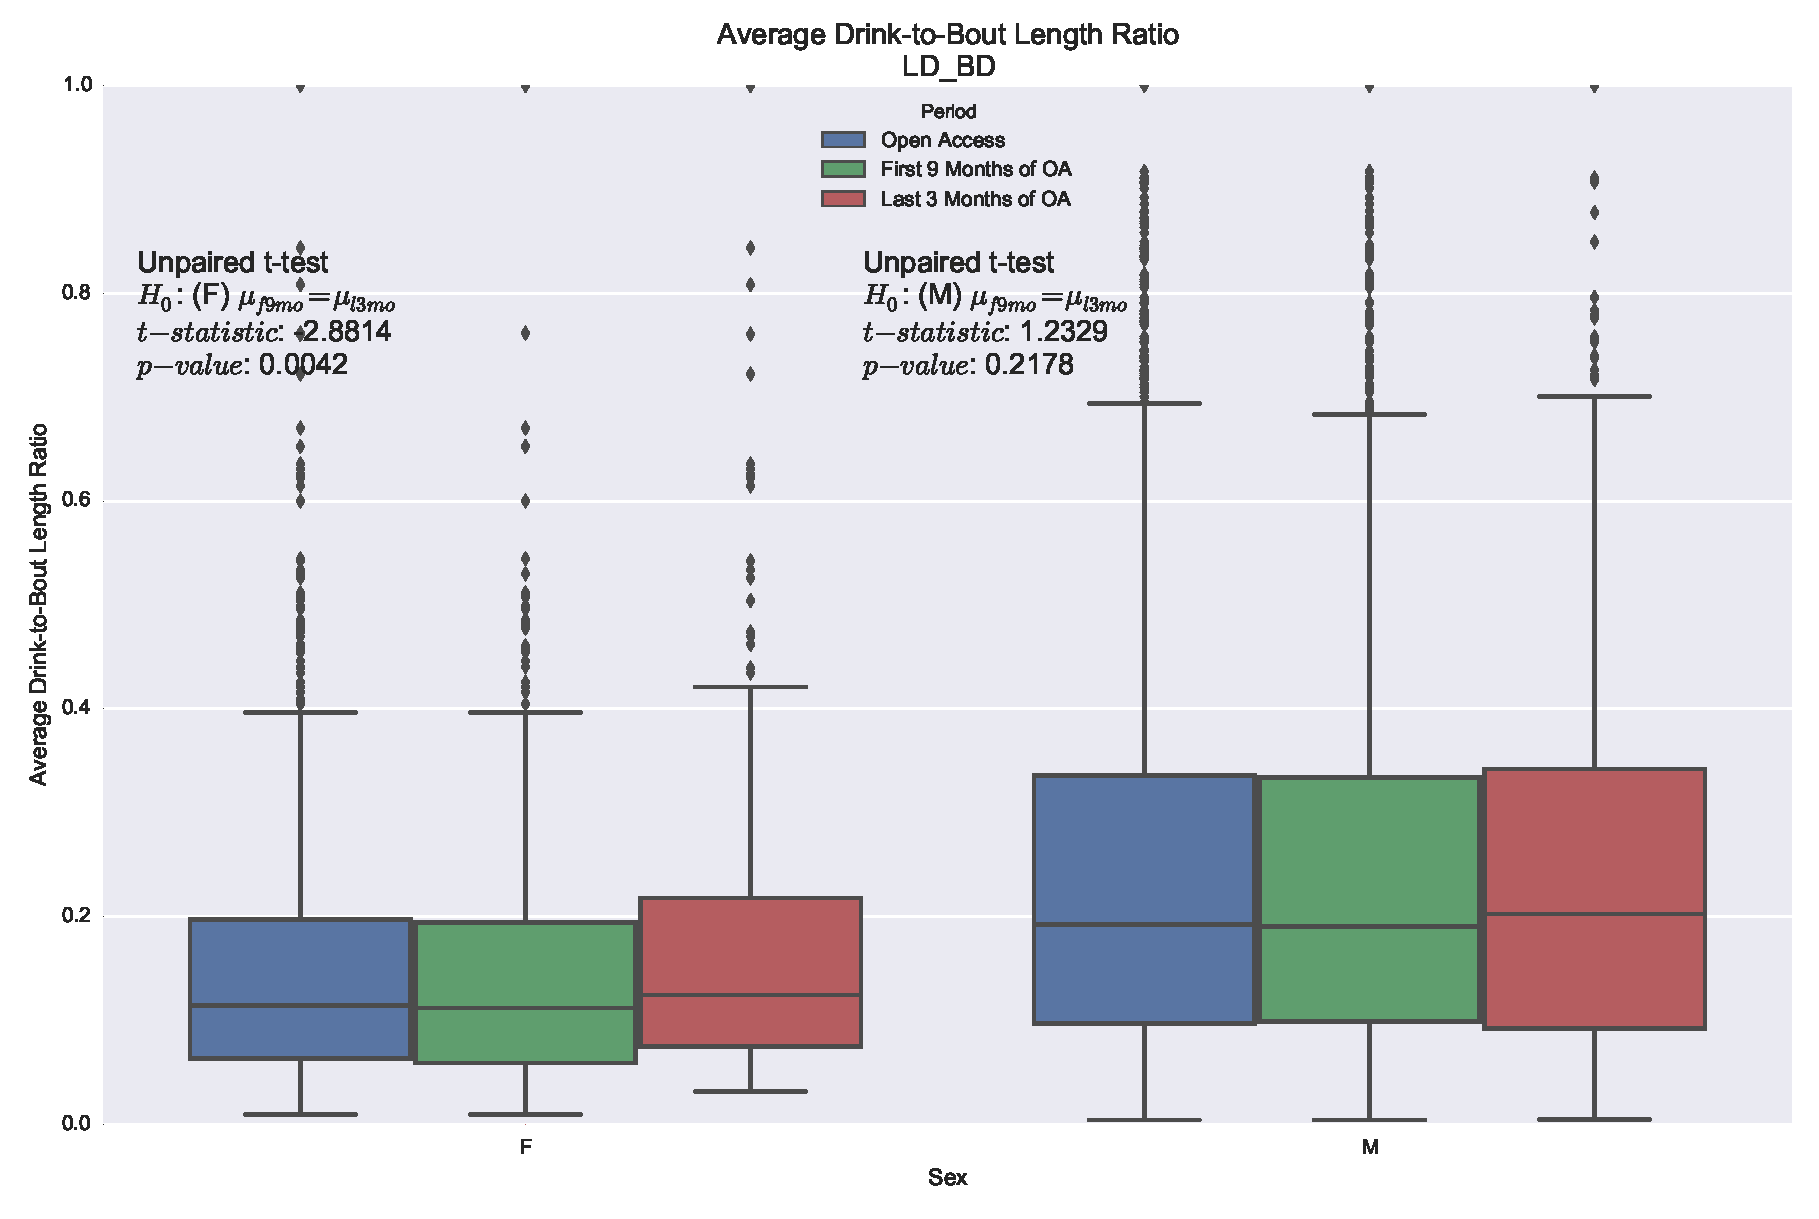
\includegraphics[width=1.1\linewidth]{figures/habitual_boxplots_mf_ttest.pdf}
		\caption{Habitual drinking factor boxplot shows the change in daily average ``drink-bout ratio" (green to red; blue - total) in both male and female populations. A t-test is used to check statistical significance of  changes.}
		\label{fig:habitual-boxplots-mf}
	\end{figure}
	
	Figure~\ref{fig:habitual-boxplots-mf}, created for low and binge drinking animals (LD \& BD), contains additional information about unpaired t-test to test the hypothesis of whether the mean value of ``drink-bout ratio" is equal for the first nine months and the last three months of the OA. There is a significant statistical difference for females but not males. In the heavy and very heavy drinking animals (HD \& VHD) the picture is reversed: there is difference in males but not females.	
	
	\begin{figure}[ht]
		\centering
		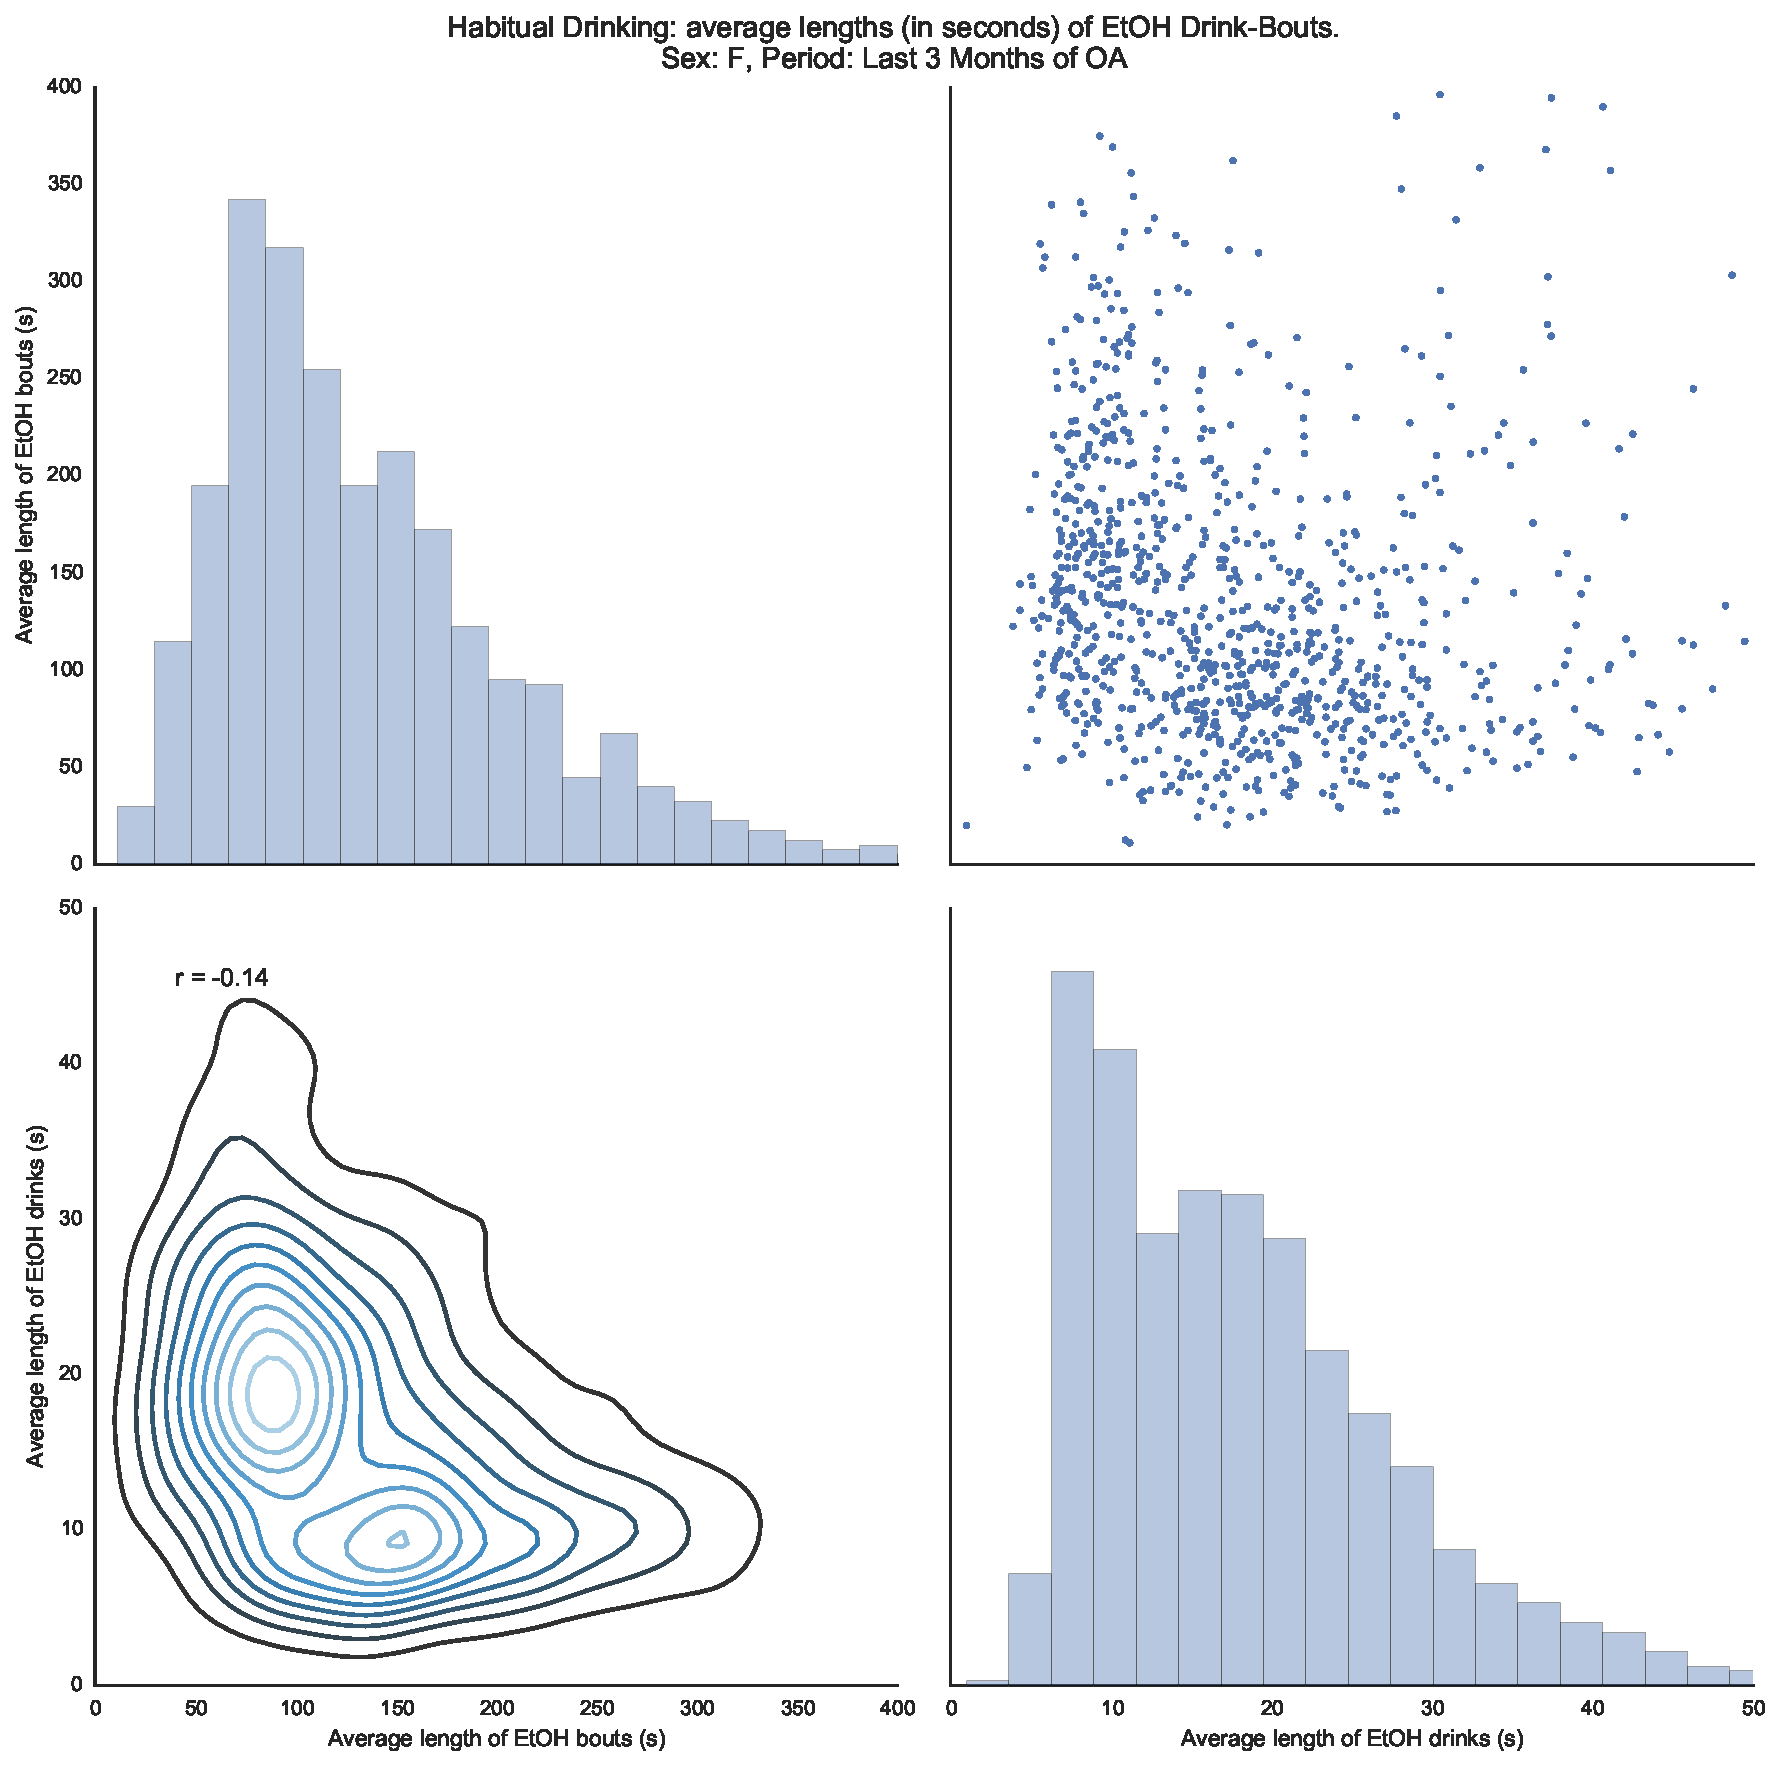
\includegraphics[width=0.85\linewidth]{figures/habitual_f_l3mo.pdf}
		\caption{Habitual drinking pair plot of the last three months of open access period for females. The X-axis represents daily average length of ethanol bouts in seconds; Y-axis shows daily average ethanol bout length. Histograms of both attributes are present on the diagonal. In the upper right corner is the scatterplot of data points for each animal per drinking day. In the lower left corner is the same data shown as a KDE plot.}
		\label{fig:habitual-l3mo-f}
	\end{figure}
	
	After we confirmed that ``drink-bout ratio" helps explain variation in the data, we decided to explore that attribute further. A pairplot captures the relationship between drinks and bouts precisely, as shown in Figure~\ref{fig:habitual-l3mo-f}. As with the boxplots, figures were created for each gender, drinking category and time period, allowing us to track data differences visually.  
	
	Figure~\ref{fig:habitual-l3mo-f} is a pairplot for female population during the last three month of OA. While histograms for each attribute show the anticipated distribution, the main diagonal of the scatterplot appears to be more sparse than the zones along the axis. To facilitate better visual perception, KDE smoothing of the multiple data points is used to plot contours of this bivariate distribution. KDE plots reveal two modes\footnote{In statistics, modes are the most frequently occuring values.} in the drink-to-bout relationship - a characteristic that is not initially (first nine months of OA) present in females and not present in males at all. 	


	
	\subsection{Menstrual Cycle Affecting Alcohol Consumption \label{section:mense}}
	The next study demonstrates how aligning and correlating data from different sources can show complex reoccurring characteristics of primate drinking, namely how the menstrual cycle affects alcohol consumption in female population. The base of the Figure~\ref{fig:mense} is a scatterplot (green dots) of the daily total ethanol intake (primary left Y-axis) during open access for one animal. To improve visual perception of the ethanol intake and to see the trend by smoothing the oscillation we applied the locally weighted linear regression technique (resulted in the green line), as explained in \cref{lwlr}. Additionally, days of the menstruation are shown with the transparent vertical red rectangles.
	
	Progesterone is a sex hormone involved in the menstrual cycle, pregnancy, and embryogenesis of humans and other species \shortcite{king2010pharmacology}. The level of progesterone in blood was measured every two to four days in female cohort ``6a". These values are plotted as dots connected by lines on top of the basis layer with secondary (right) Y-axis indicating the exact amount. The correlation between the hormone level and smoothed drinking osculations is now accessible by the naked eye: this heavy drinking female is drinking notably more a few days after peak progesterone.   
	
	\begin{figure}[ht]
		\makebox[\textwidth][c]{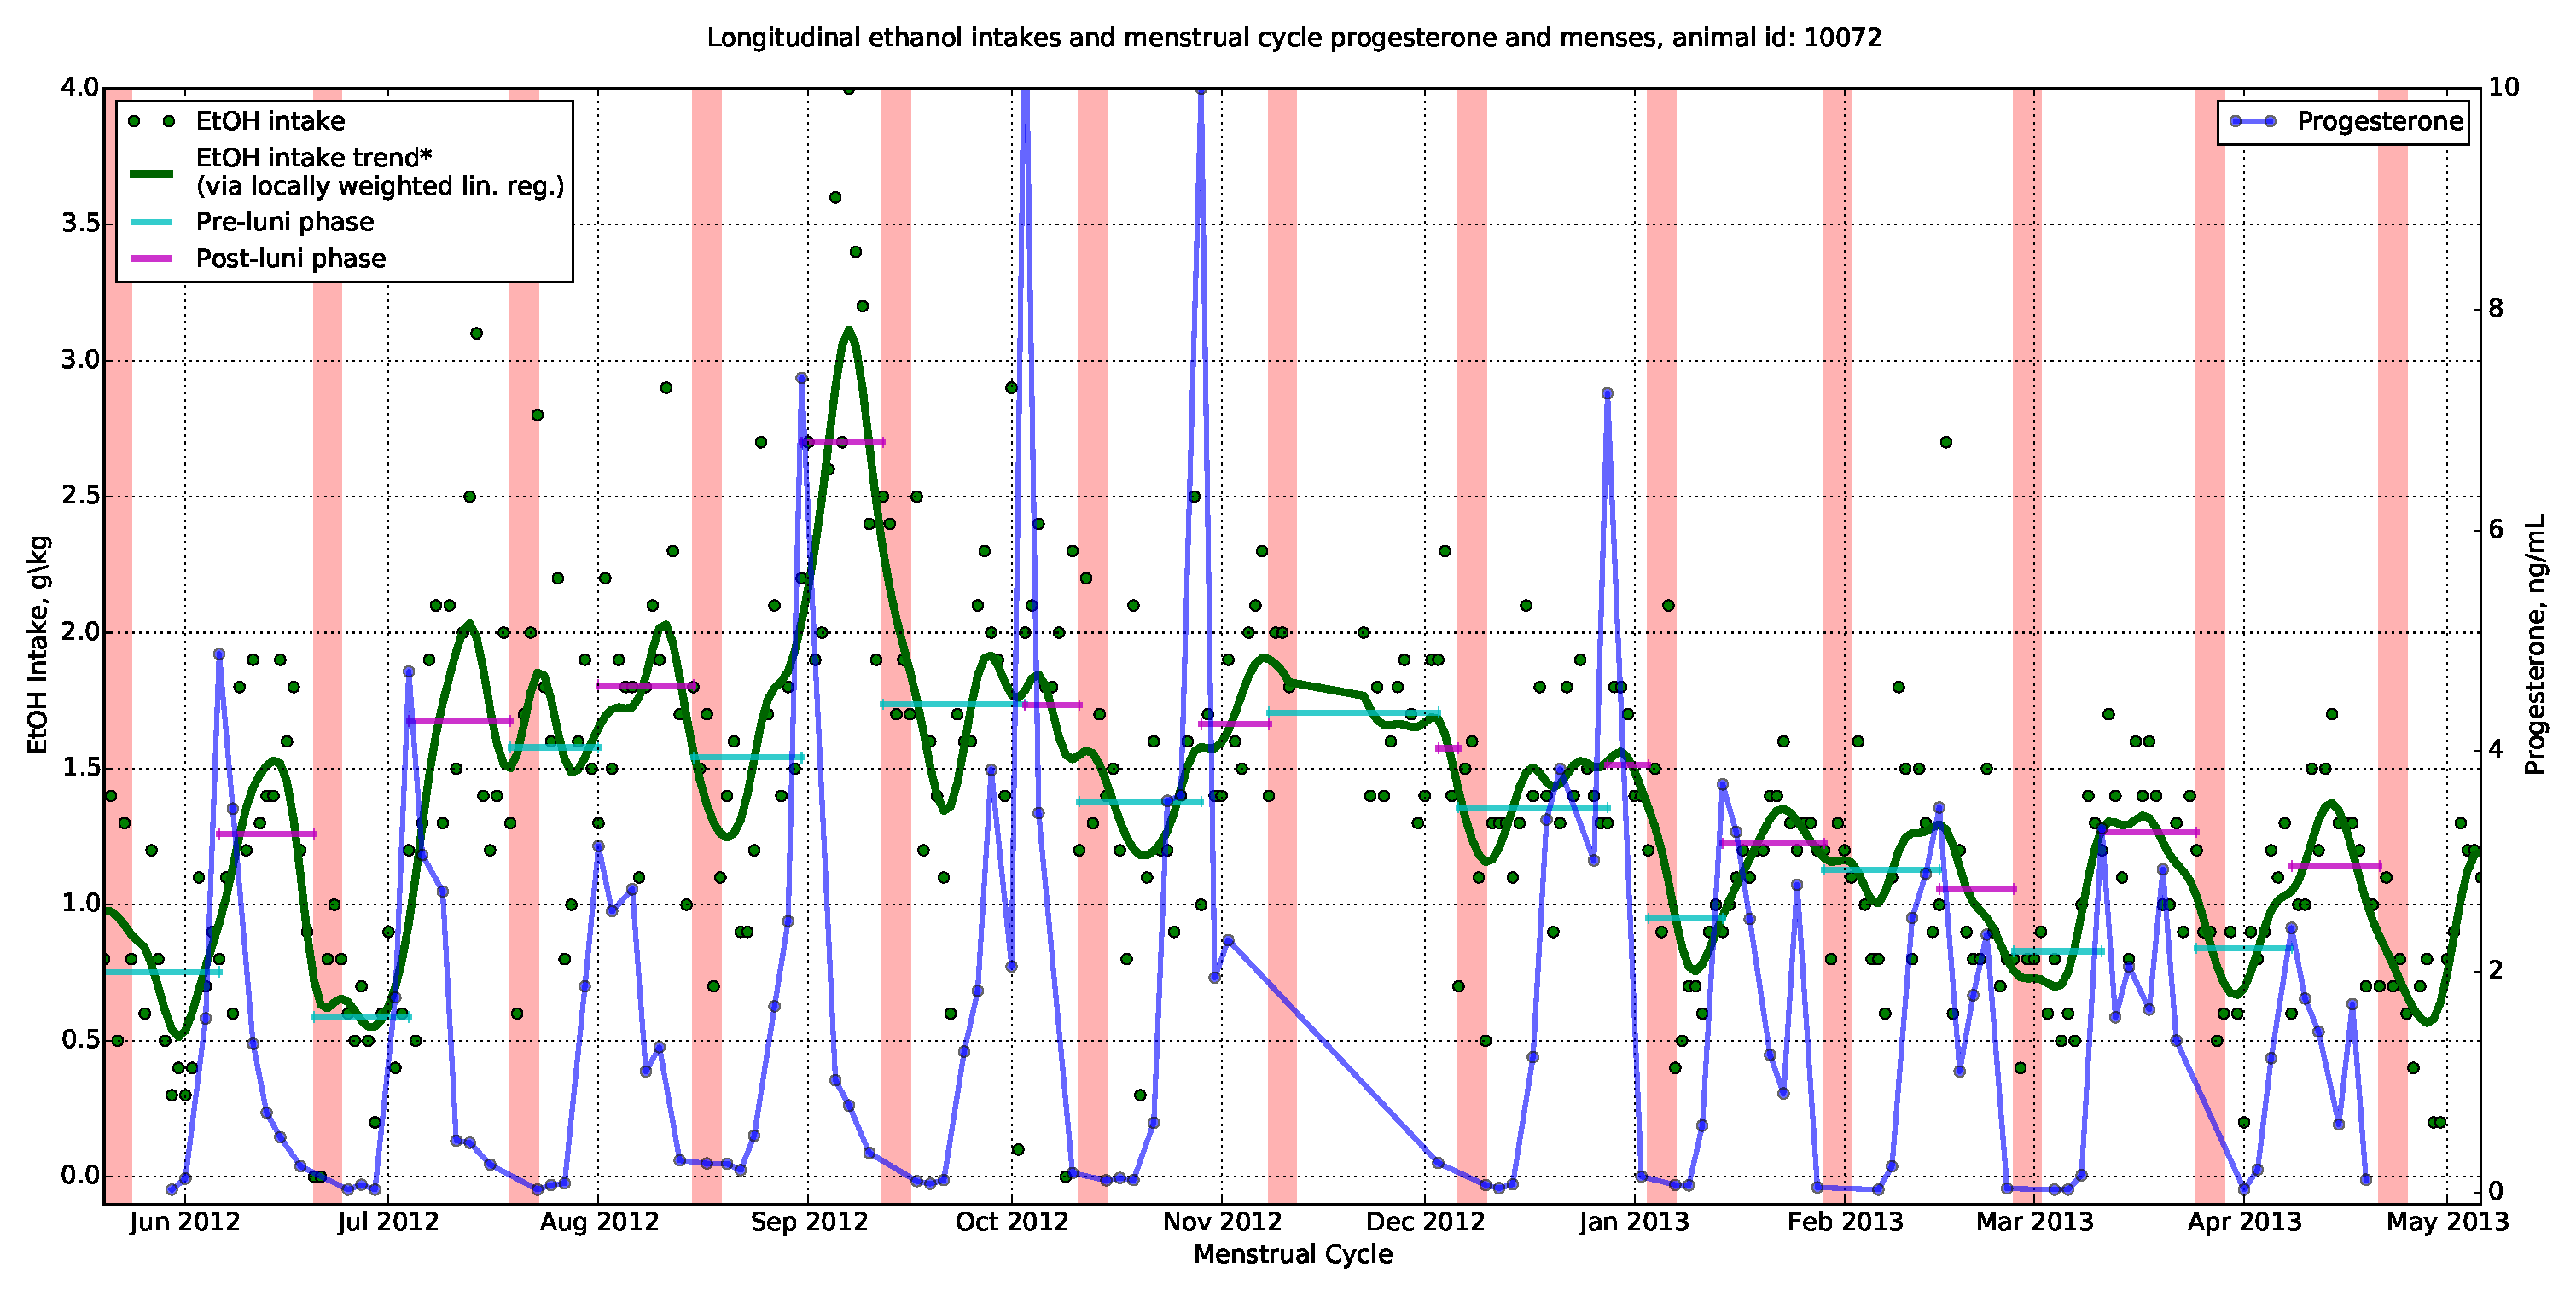
\includegraphics[width=1.3\textwidth]{figures/mense_progesterone_oa.pdf}}
		%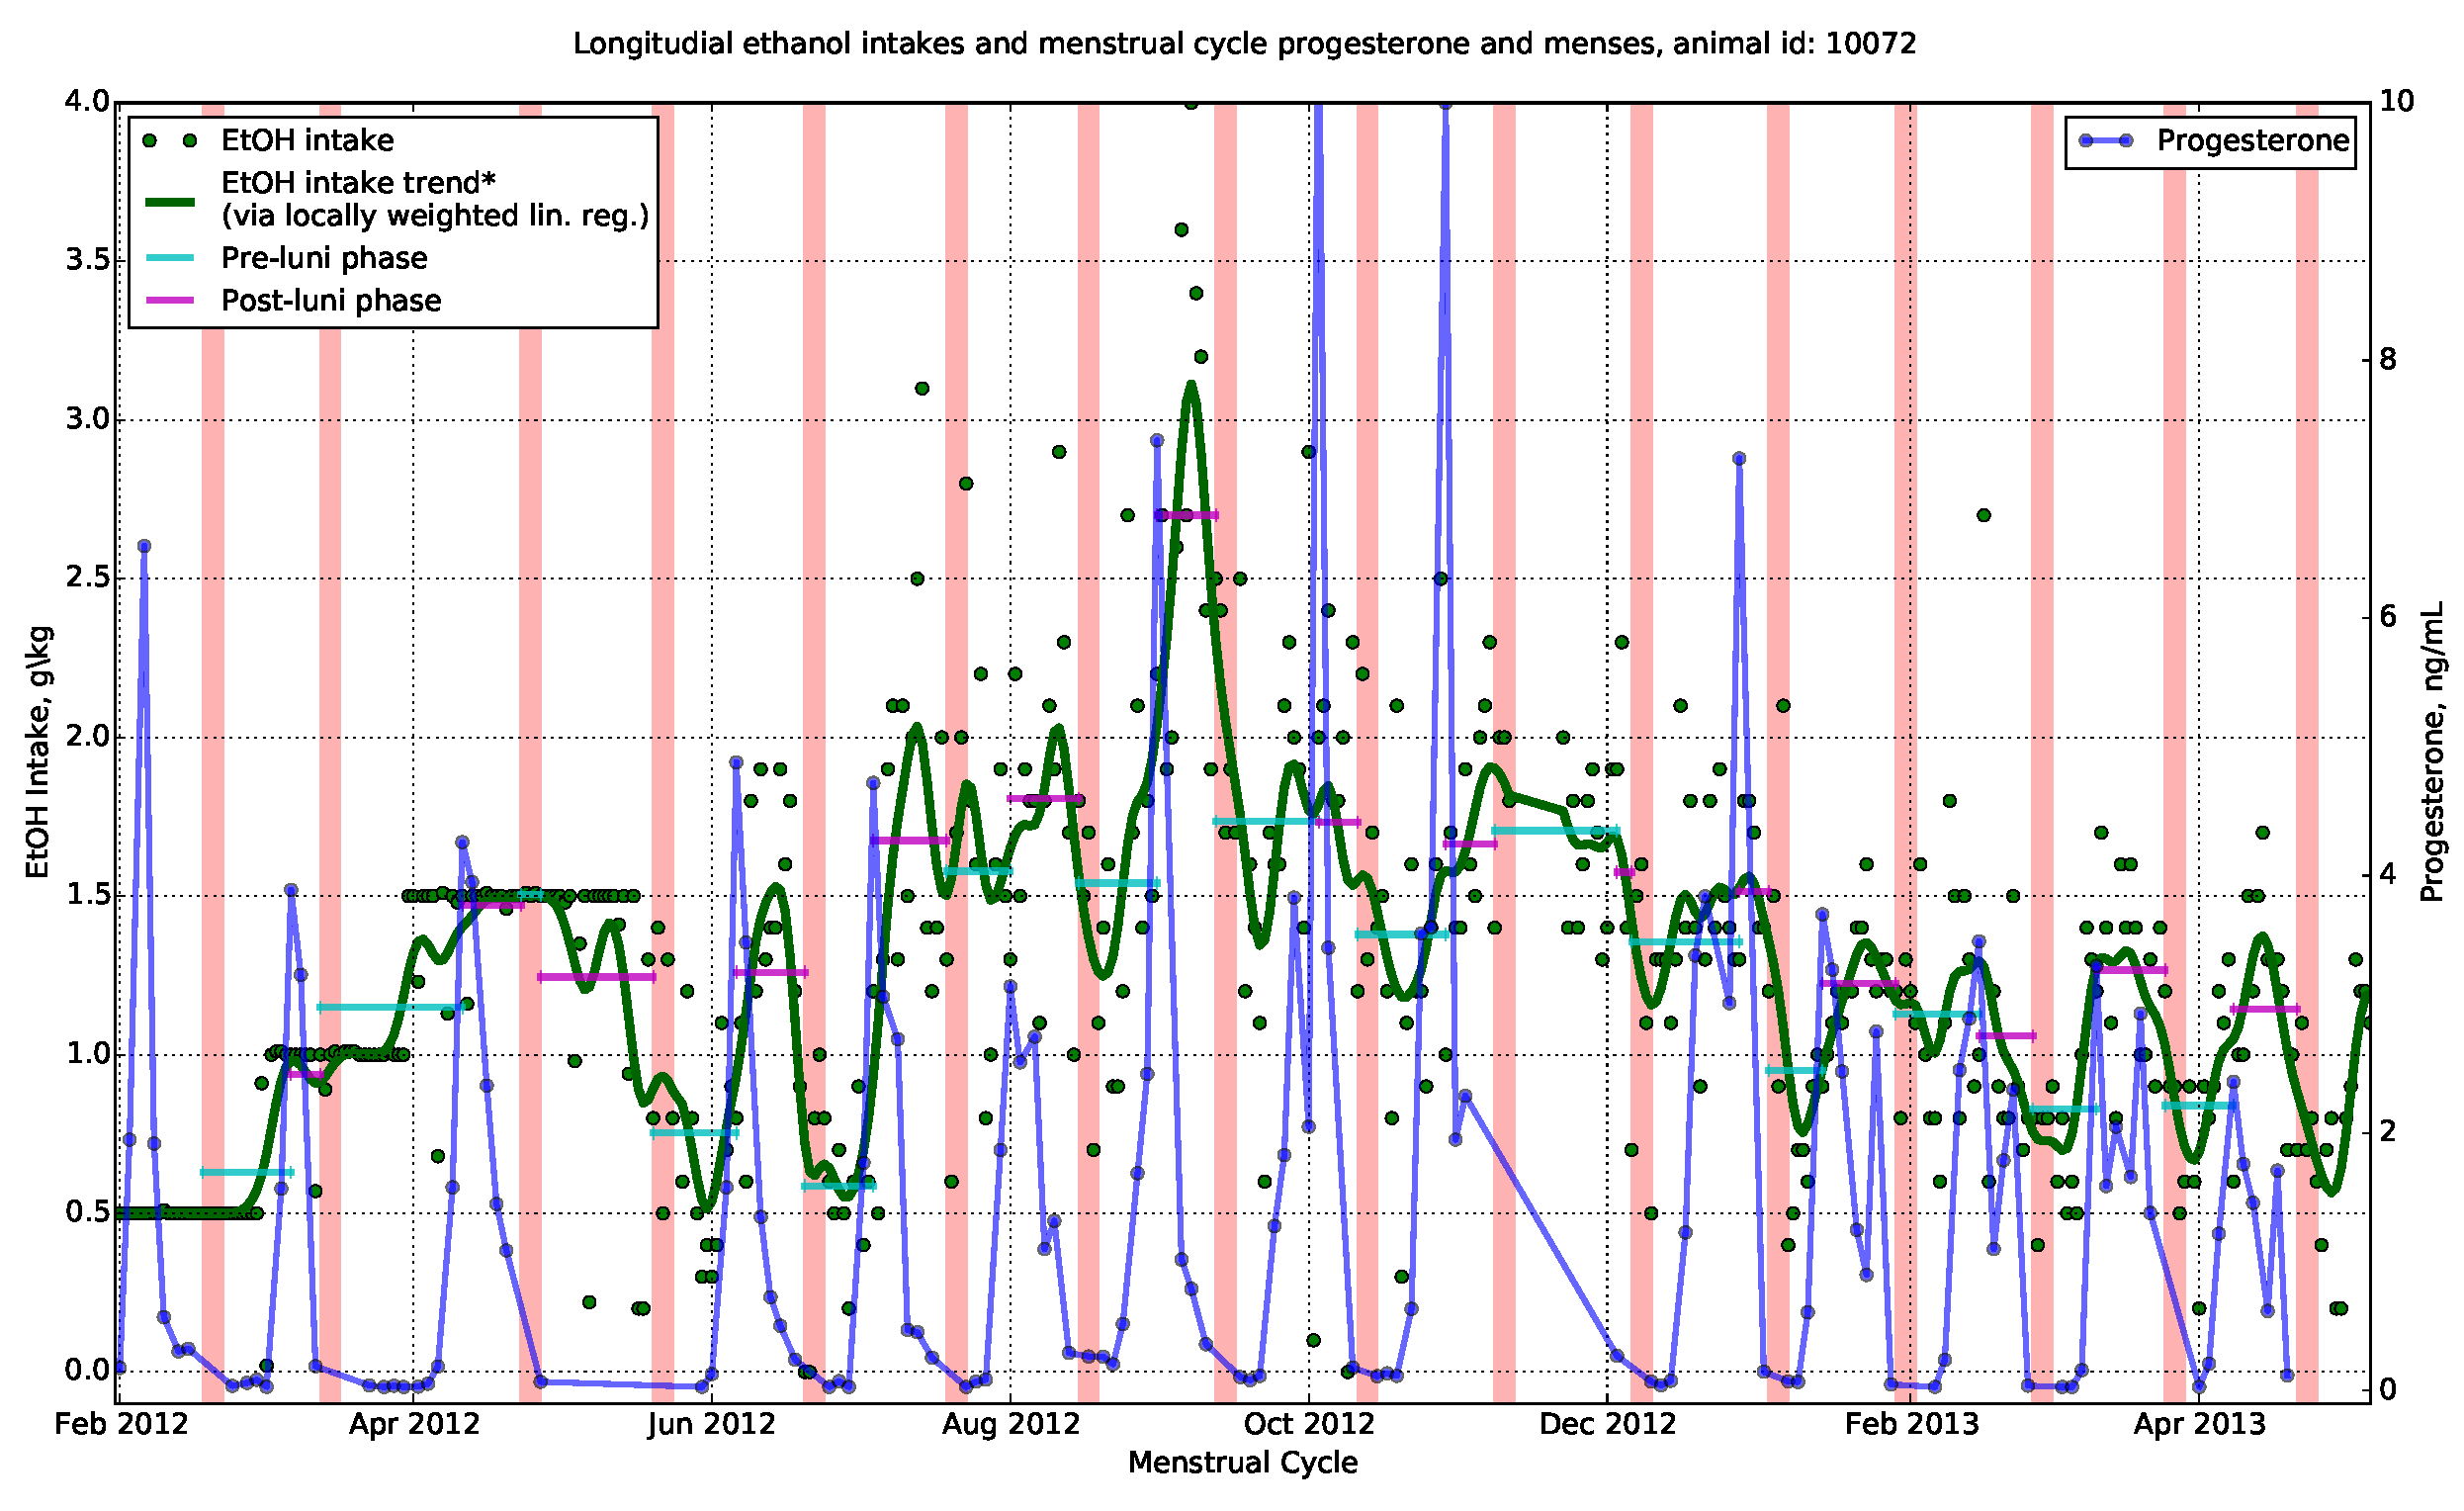
\includegraphics[width=1.3\linewidth]{figures/mense_progesterone.pdf}
		\caption{Menstruation cycle influence on ethanol intake. Vertical red rectangles depict days of  menstruation by date in the X-axis. Dots represent daily EtOH consumed as average in g/kg. The green line shows the smoothed trend obtained via locally weighted linear regression; the blue line connects the points of progesterone level observations. There is a visual correlation between green and blue lines. Cyan and purple horizontal lines show pre-luni and post-luni menstrual phases, respectively.}
		\label{fig:mense}
	\end{figure}
	
	To extend the analysis of how much this animal's drinking changes, on average, we first divide all the ethanol intake data points by full menstrual cycle. Then, within each cycle, we divide data points into two phases: pre-luni and post-luni. Pre-luni phase starts with the beginning of the cycle and ends when the progesterone level is in the highest (peak in the blue line). Post-luni begins here and ends with the start of new cycle. For each pre-luni and post-luni phase within each cycle the average ethanol intake was calculated and plotted as a horizontal lines (cyan and purple colors, respectively). In every case but one the level of average ethanol intake is much higher during the post-luni phase then during the pre-luni phase which indicates the direct influence of female hormones on the alcohol consumption. 
	

	\subsection{BEC $\sim$ EtOH Correlation}	
	Throughout the ethanol self-administration experiment there were regular (every fifth day) blood drawings  that track the Blood Ethanol Concentration (BEC) levels in the subjects. The BEC is an objective measurement of intoxication. However, there are some issues too: since blood is drawn only once every five days at an arbitrary time it may be the case that some animals, preferring morning drinking, are already getting sober, while others, preferring night drinking, have not yet started their alcohol consumption. Hence this study aims to investigate the reliability of the BEC as well as to look for anomalies and specific patterns. One particular pattern was watched for: do animals from different drinking categories drink differently the day after hard alcohol intoxication (defined as above a certain level of BEC)? Below is a description of the study along with the results, implications and limitations. 
	
	First, we gathered the BEC data from regular samples from available cohorts\footnote{Few cohorts do not provide BEC data.} resulting in nearly 6000 rows containing animal id, date and time of sample, and the BEC in form of milligram percentage (mg \%). Then the ethanol consumed up to the sample time that day was calculated for each animal (EtOH day of BEC sample). Then values for the total ethanol consumed the days before and after the BEC sample were retrieved (EtOH day before and EtOH day after, respectively); days with exceptions in either BEC or EtOH data were filtered out.
	
	\begin{figure}[ht]
		\centering
		\makebox[\textwidth][c]{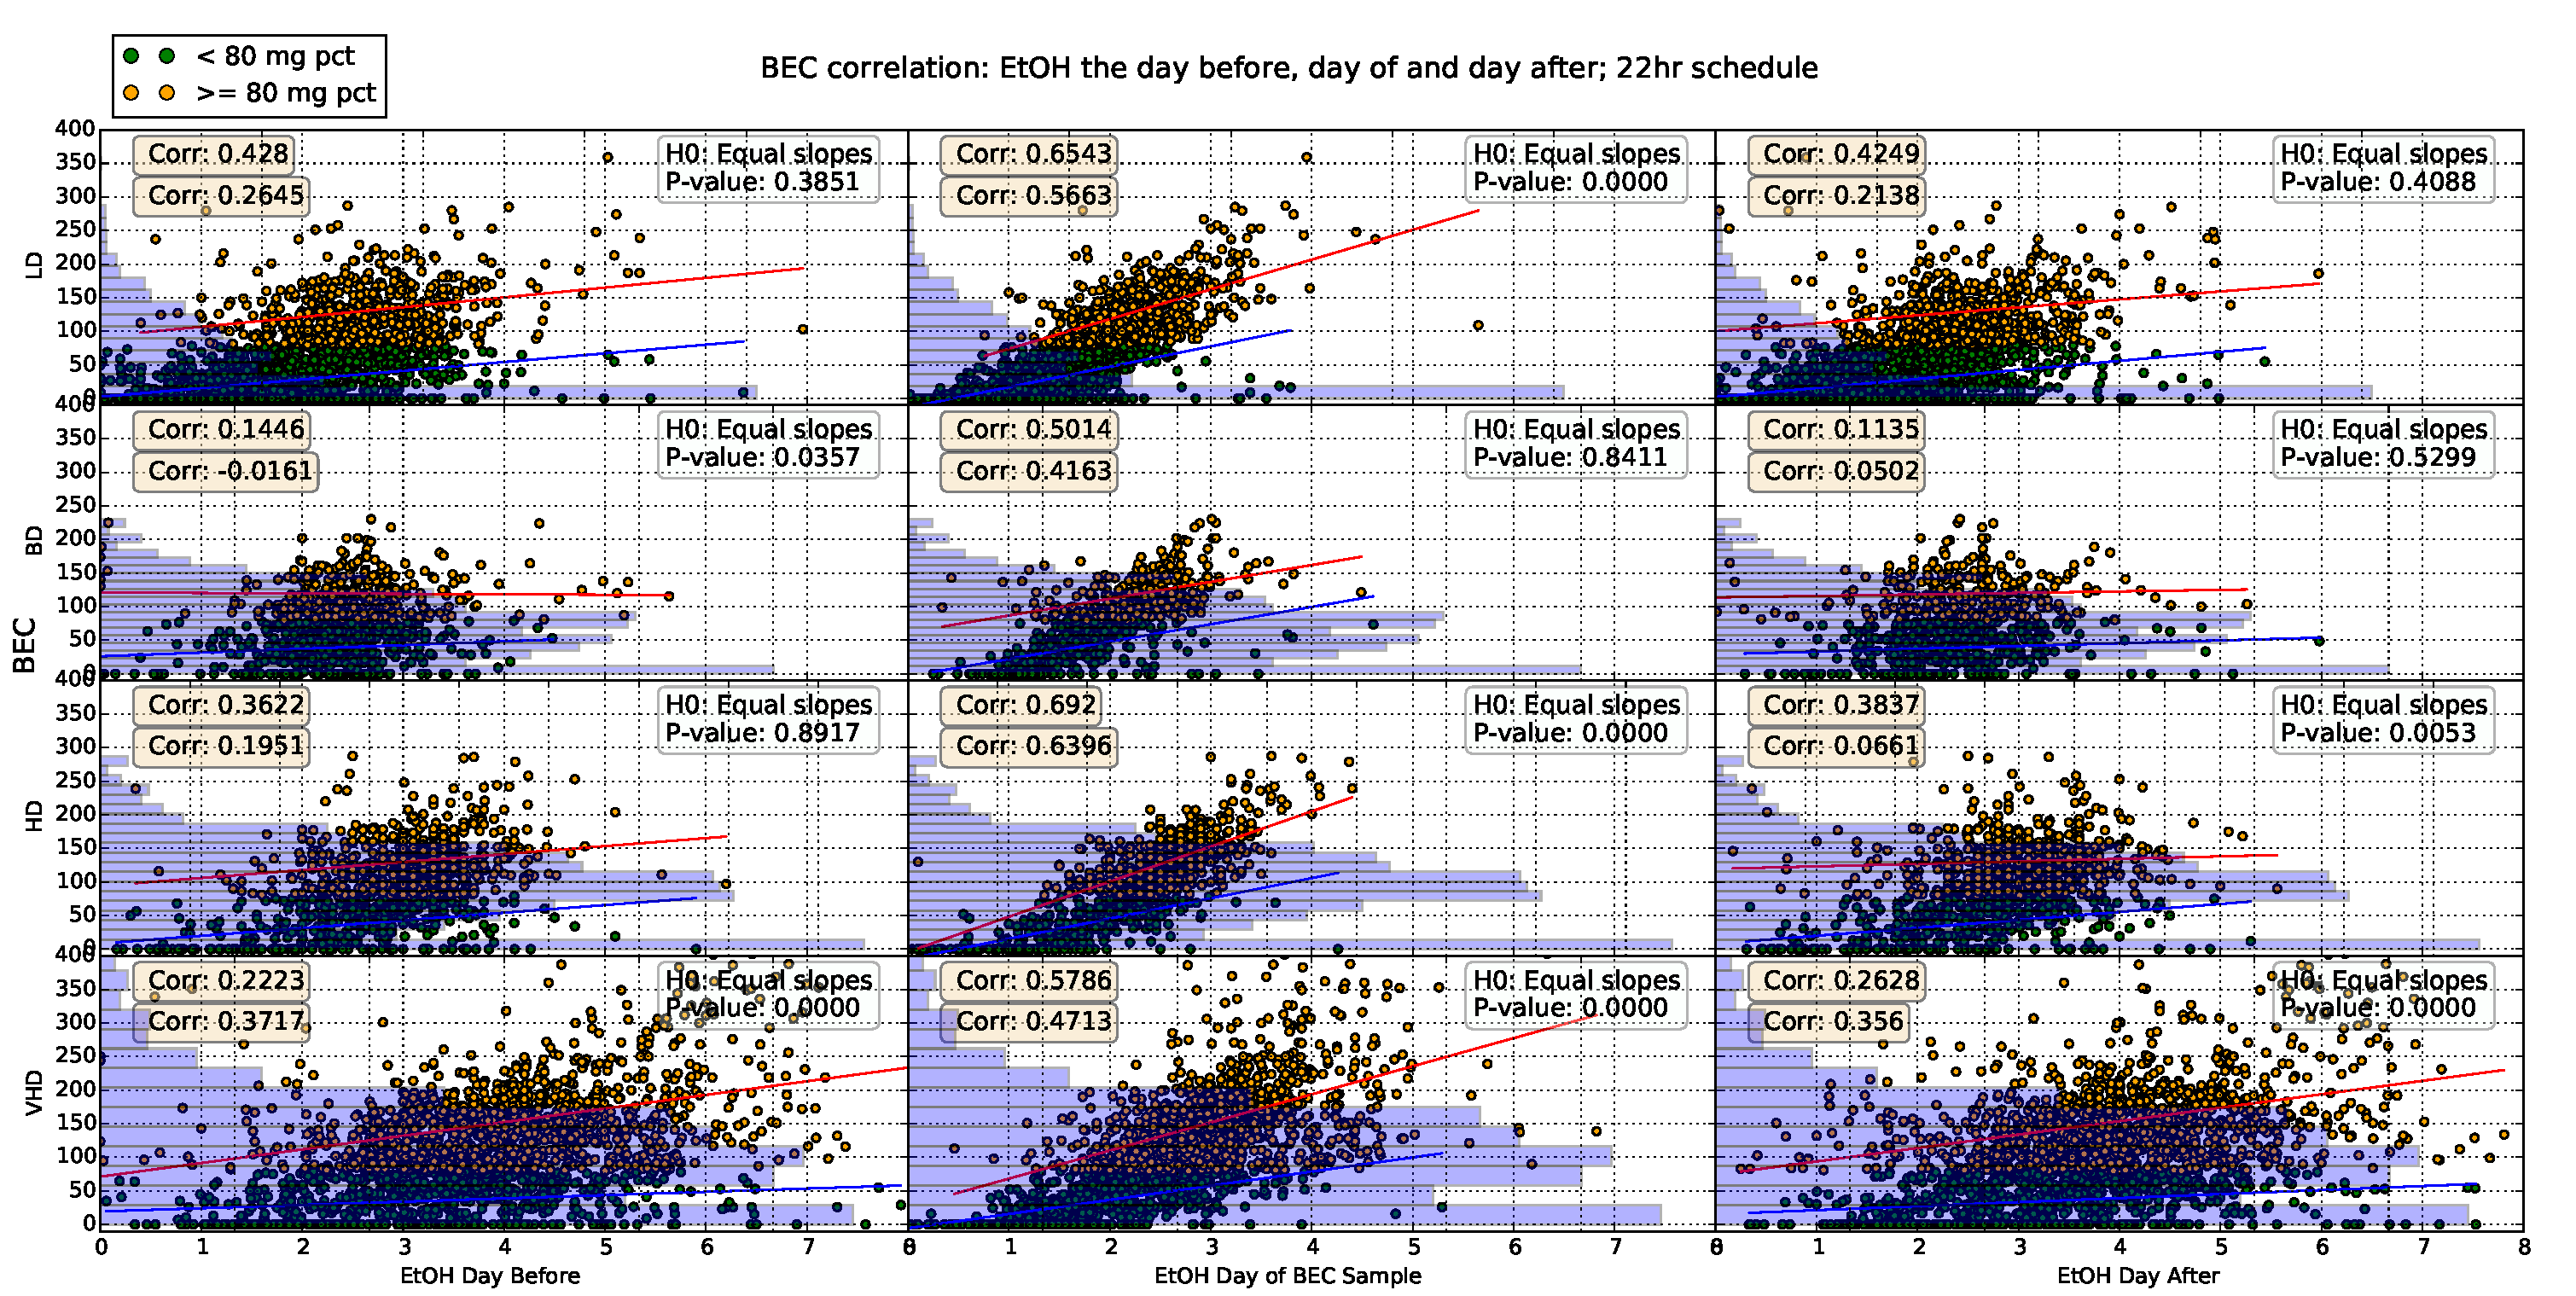
\includegraphics[width=1.2\textwidth]{figures/bec_etoh_over80mg_22hr.pdf}}
		\caption{Combined BEC $\sim$ EtOH correlation plot for all animals displaying a grid of panels: four rows by drinking category, three columns with ethanol the day before, the day of and the day after the BEC sample. On each panel Y-axis represents the level of BEC (mg \%) the day of sample. The X-axis represents the ethanol consumed by the animal: total EtOH the day before BEC sample in the left column, total EtOH up to the sample time at the middle column and total EtOH the day after BEC sample in the right column. Each panel describes the ethanol versus sample BEC, divided into two groups (less or more than 80 mg pct BEC) and contains: scatter plot of EtOH$\sim$ BEC; sample's BEC values overlaid as histogram (grouped by drinking category); Pearson correlation product for each group; linear regression fit lines and ANCOVA p-value testing whether those two lines have equal slopes.    }
		\label{fig:bec-over80}
	\end{figure}
	
	At this point we had approximately 5500 data points with the following information: animal id, drinking category, sample BEC level, EtOH day before, EtOH day of BEC sample and EtOH day after. Ultimately, we wanted to see and measure the correlation between ethanol consumed at one of the three consecutive days and BEC level at each slice of the qualitative attributes. Additionally, we wanted to see if the intoxication event plays a role and divided all data points into two groups: BEC at intoxication level equal or over 80 mg \% or not. 
	
	Visual representation of the results is shown on the Figure~\ref{fig:bec-over80} containing a grid of panels. Rows separate drinking categories and columns represent EtOH the day before, day of and day after the BEC sample. Each panel has a scatterplot of data points described above. Points of intoxication are shown in orange. Surprisingly, low drinking animals appear to have elevated numbers of intoxication events. In fact, \textit{it seems} they have the same number of the orange points as the heavy drinking animals. This is, however, due to the high density of points, which skews the visual perception. By looking at the overlaid normed histograms of the BEC values for each drinking category we can see that intoxication, as defined here, is much more likely among VHDs than LDs.   
		
	Each panel on Figure~\ref{fig:bec-over80} also contains a Pearson correlation value and linear regression fit lines for each group, as well as the ANCOVA p-value for the hypothesis testing whether those two lines have equal slopes. First consider low drinking animals. Statistically (ANCOVA p-value) two groups (intoxicated or not) have a different line of ethanol consumption up to the BEC sample time, while the day before and the day after two groups do not differ. In binge drinking animals, two groups drink differently during the day before intoxication, but not the day of and the day after the sample. That may be an indicator that in BDs there is a factor today that causes the occasional drink tomorrow. In heavy drinkers the pattern is reversed: two groups drink similarly the day before intoxication, but differently the day of and the day after. That may indicate that once intoxicated HDs can not stop drinking, hence such divergence. In very heavy drinkers, coherently with the interpretation of HDs, two groups drink differently all three consecutive days, which may indicate that for them the intoxication becomes a vicious cycle. 

	While defining intoxication as over 80 \% BEC is a widely accepted method, it has limitations. For example, the ANCOVA model implies the assumption that the covariate is independent of the treatment effects. In our case it is not entirely true since we split the data based on the BEC level. Additionally, it may seem unfair to call two animals from \textit{different drinking categories} intoxicated after achieving the \textit{same level of BEC}. The alternative is to define alcohol intoxication for the animal as an event of ethanol consumption over an arbitrary threshold number of standard deviations \textit{for that particular animal}. The later part of this study adopts this definition with the threshold equal two\footnote{We do not use the lower threshold because there are a lot of zero BEC measurements due to the various reasons.}. Thus for each animal the intoxication is defined as EtOH consumed is over two standard deviations above the mean:
	\begin{equation} \label{eq:intox-std}
	\mathbbm{1}{ \{x > \mu + 2*\hat{s}\}}
	\end{equation} 
	
	As shown on Figure~\ref{fig:bec-over80}, besides incorporating the new definition, we alleviate the problem of high density scatterplots by using hexagonal bin (hexbin) plots.
	\begin{figure}[ht]
		\centering
		\makebox[\textwidth][c]{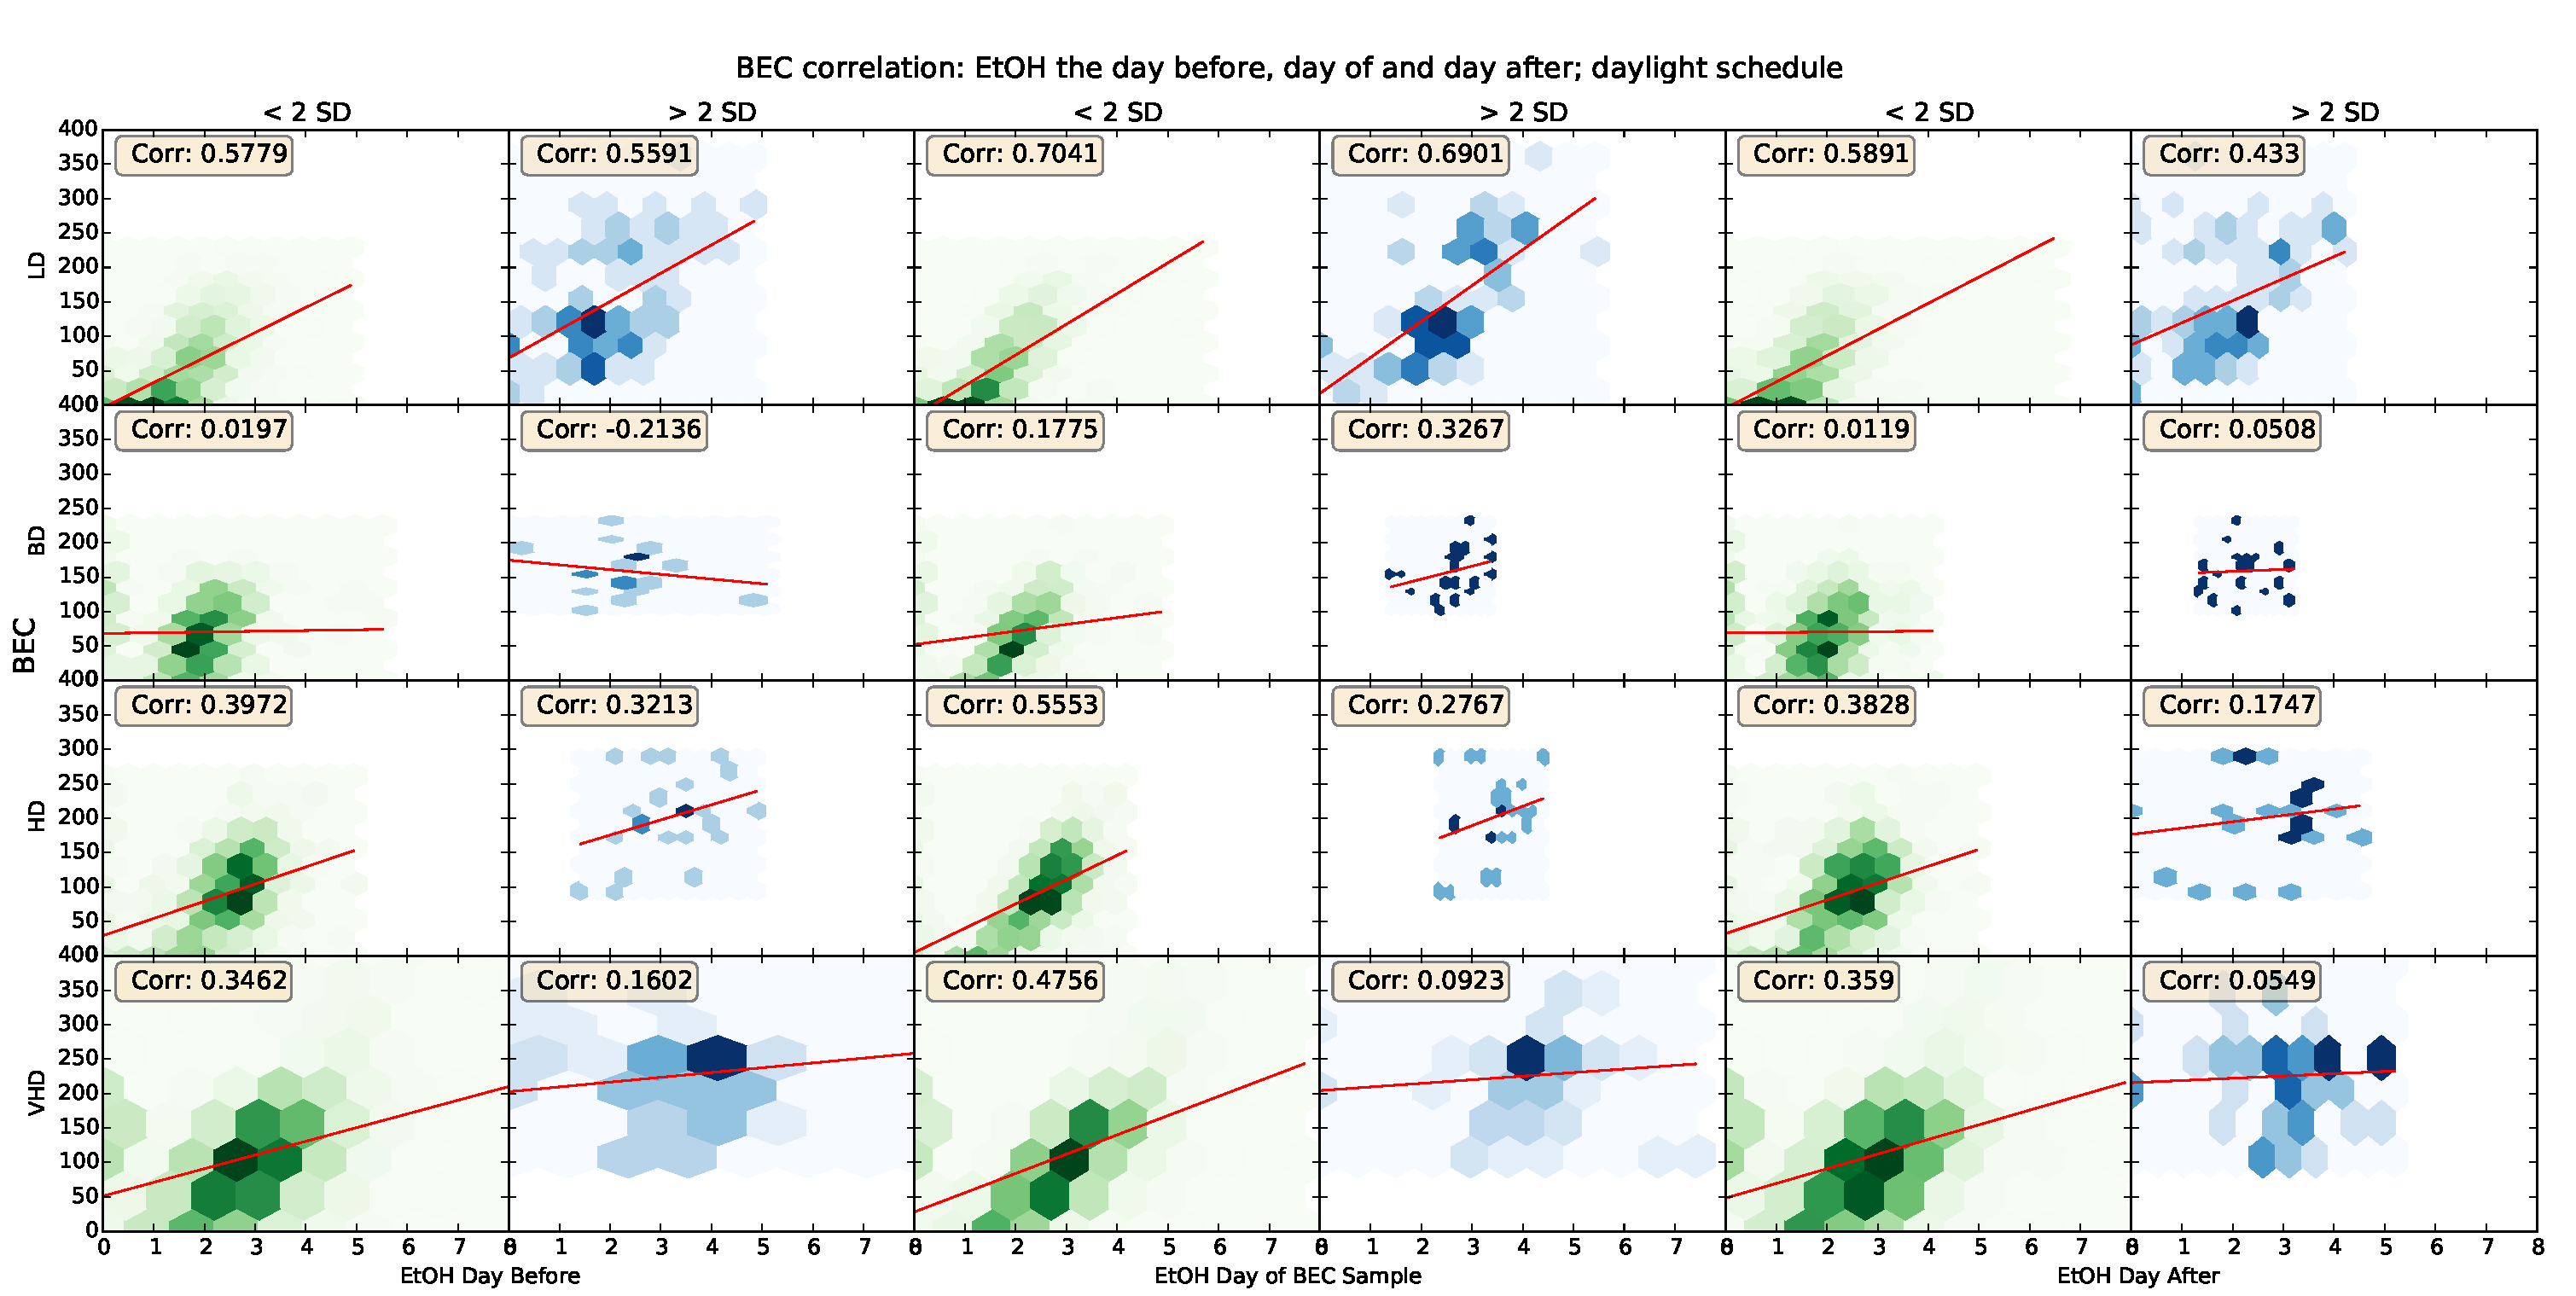
\includegraphics[width=1.2\textwidth]{figures/bec_etoh_more2std_daylight.pdf}}
		\caption{BEC $\sim$ EtOH correlation hexbin plots containing 24 panels for each DC the day before, day of and the day after BEC sample, split by intoxication event; Person correlation and linear regression fit lines are overlaid on each panel.}
		\label{fig:bec-more80}
	\end{figure}
	
	The hexbin plot could be thought of as 2D histogram and allows us to reduce the density of the data. Since it is hard to overlay the hexbin plots we now provide 24 separate panels rather than 12 combined panels. Additionally, in Figure~\ref{fig:bec-over80} we used data sorted by the \textit{daylight schedule}, which adds two hours of the last day's session. It is conjectured that animals start activities when the lab employees come to work, which happens before the lights are turned on. 
	
	First consider the correlation between the BEC level and EtOH at the sample time. On typical drinking days (no intoxication), low drinking animals (LDs) show the highest correlation, which may indicate that \textit{they do not drink much after the BEC sample}, while BDs show the least correlation, which may indicate the \textit{sporadic nature} of their drinking. On intoxication days, correlation values are less for all drinking categories, and almost not visible for VHDs, which may indicate that animals either drink much before sample (getting sober by the BEC sample time) or drink much after the sample (since VHDs have problems with stopping) - in either case BEC measurement \textit{fails to capture the true state of alcohol consumption}.
	
	Now consider Binge Drinkers (BDs). As expected, on typical drinking days with no intoxication, there is essentially \textit{no correlation} between the EtOH the day before, the day after and the BEC the day of sample is. However, on intoxication days, the amount of the ethanol consumed the day before is \textit{negatively correlated} with the BEC level the day of sample, which may indicate the effect of disliking alcohol side effects: \textit{BD animals that drunk a bit too much yesterday do not want to get intoxicated today}. 
	
	\subsection{Drinking The Day After Intoxication}
	As an extension of the BEC $\sim$ EtOH correlation study we decided to analyze the drinking the day after intoxication for all the data points available in the same males (cohorts ``5", ``7a" and ``7b") and females (cohorts ``6a" and ``6b") populations. Rather than BEC we now rely on abnormally high (for individual animal) total ethanol consumption as a measurement of the intoxication. 
	
	The first step is to find the intoxication days. Out of all drinking days (roughly eleven thousand total), days of intoxication were found as days with consumption over $\gamma$ standard deviations, for each individual animal. After trying various values for the parameter $\gamma$, it is found that the most illustrious values are in the range between 1.5 and 2. These values of $\gamma$ rendered approximately two to six percent of the days to be the intoxication days, on average.
	
	\begin{figure}[ht]
		\centering
		\makebox[\textwidth][c]{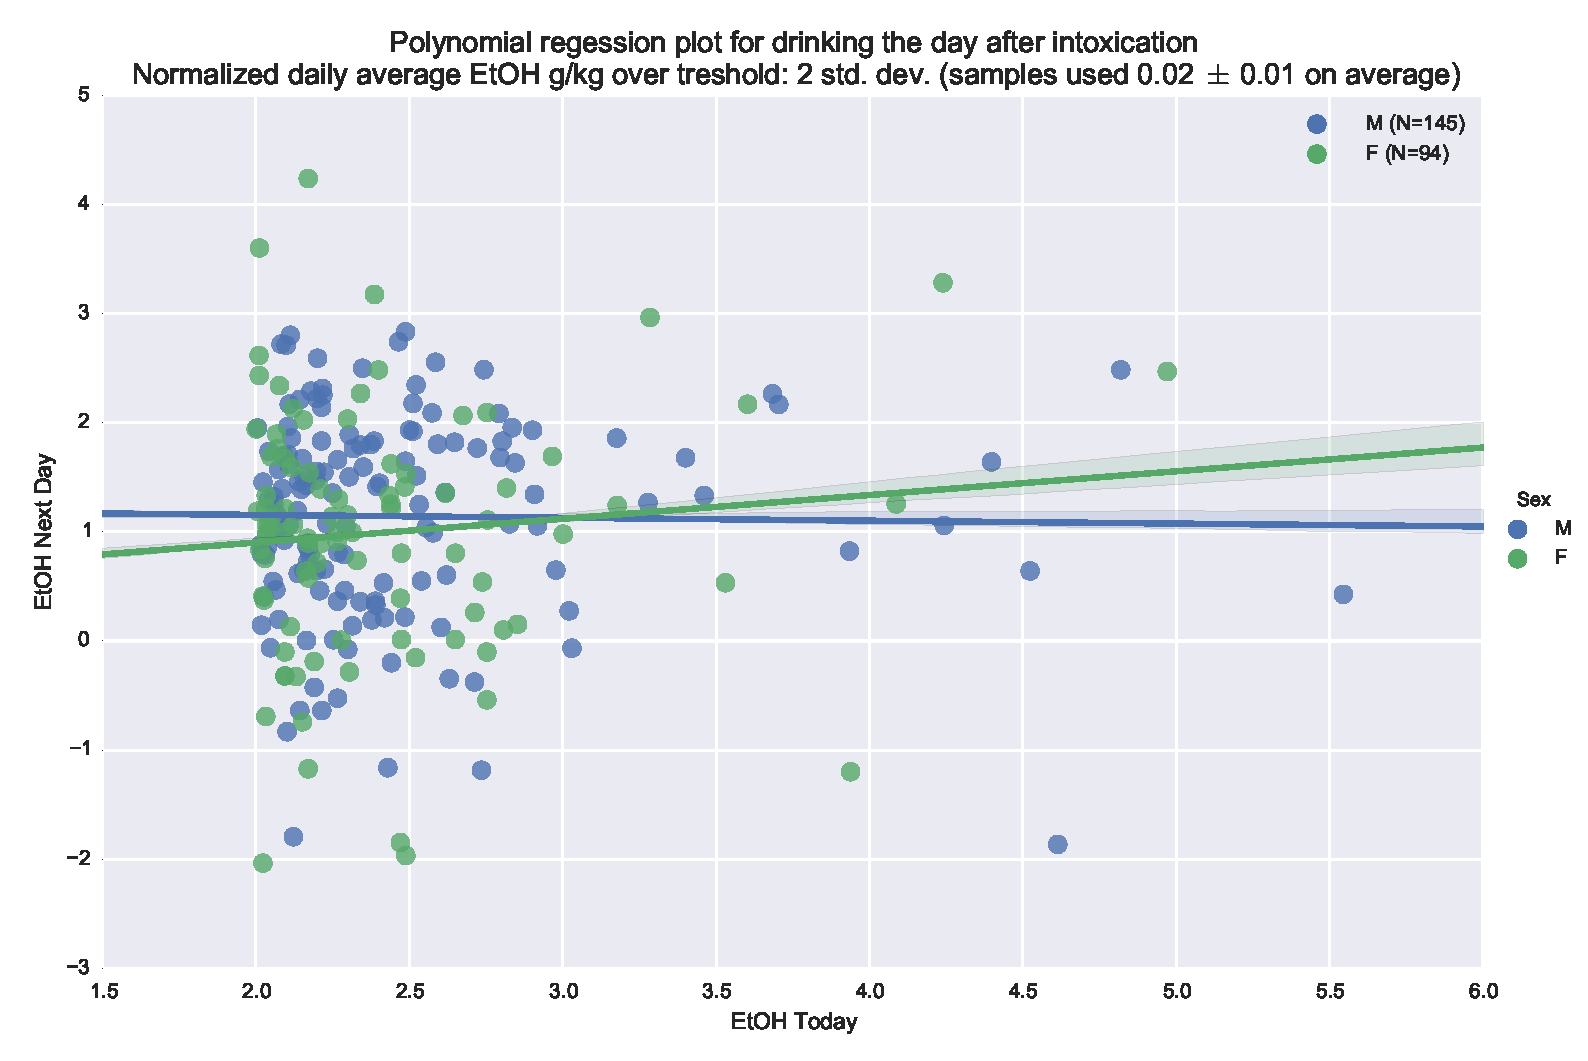
\includegraphics[width=1.1\linewidth]{figures/intox_poly-reg-factor_mf_lines.pdf}}		
		\caption{Regression plot for drinking the day after intoxication. X-axis shows the ethanol consumption (in g/kg) the day of the intoxication; Y-axis shows consumption the day after. With gender as a factor, two lines are fitted into data points.}
		\label{fig:intox-poly-reg}
	\end{figure}
		
	The second step is to collect the daily total ethanol consumption in grams per kilogram of body weight (g/kg) during days that followed the days of intoxication. The factor scatterplot of such data, along with the regression fit lines are shown on Figure~\ref{fig:intox-poly-reg}. 
	
	As expected, animals of both gender greatly reduce, on average, ethanol consumption the day after intoxication. However, as illustrated by the fitted lines, females tend to have slightly more days of heavy drinking the day after intoxication, than males. This might be due to either an internal feature of the females or a third unaccounted for factor.    
	
	Another way of looking at this data is to analyze the role of the each drinking category\footnote{"BD" drinking category is not present in the female population and was not used for this part of the study.} while compressing the change (reduction) in the drinking the day after intoxication into single average point, keeping gender as a factor. The factor line plot of that is shown on Figure~\ref{fig:intox-factor-line}. 
	\begin{figure}[ht]
		\centering
		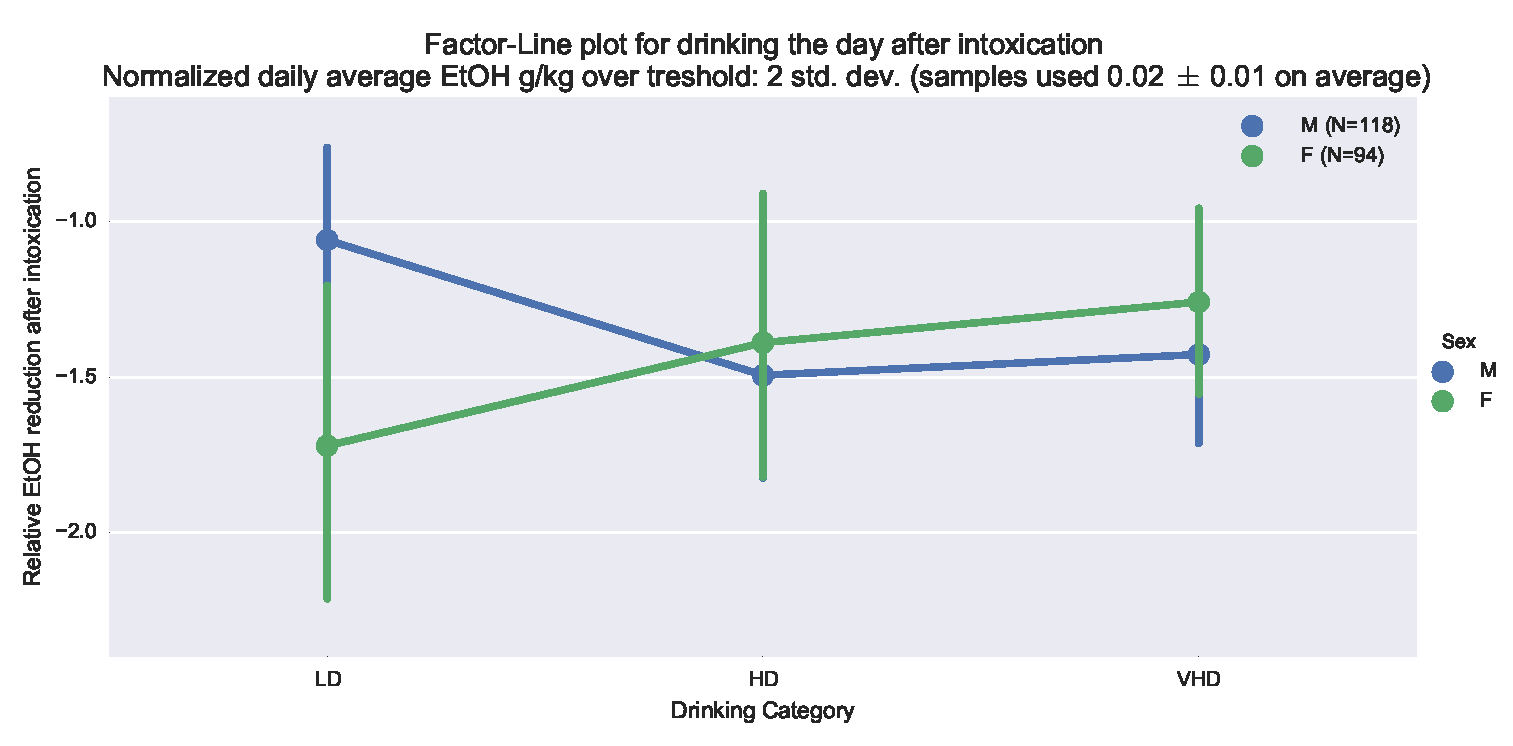
\includegraphics[width=\linewidth]{figures/intox_factor-line_mf.pdf}
		\caption{Factor-line plot for drinking the day after intoxication.  Y-axis shows the change (reduction) in drinking the day after intoxication (6\% of total drinking days), for each drinking category of X-axis.}
		\label{fig:intox-factor-line}
	\end{figure}
	
	We can see that trends are the opposite between drinking categories for two genders: very heavy drinking females tend to reduce the drinking much less the day after intoxication than low drinking ones; conversely, heavy drinking males reduce the drinking more the day after intoxication than low drinking ones.	
	
	Finally, to expand our understanding of these drinking category and gender differences in drinking after intoxication we employed violin plots. Figure~\ref{fig:intox-violin} demonstrates the distribution of the intake reduction in males and in females for each drinking category. In our case this plot does not reveal any additional information and only confirms the observations made based on the line factor plot.  	
	\begin{figure}[ht]
		\centering
		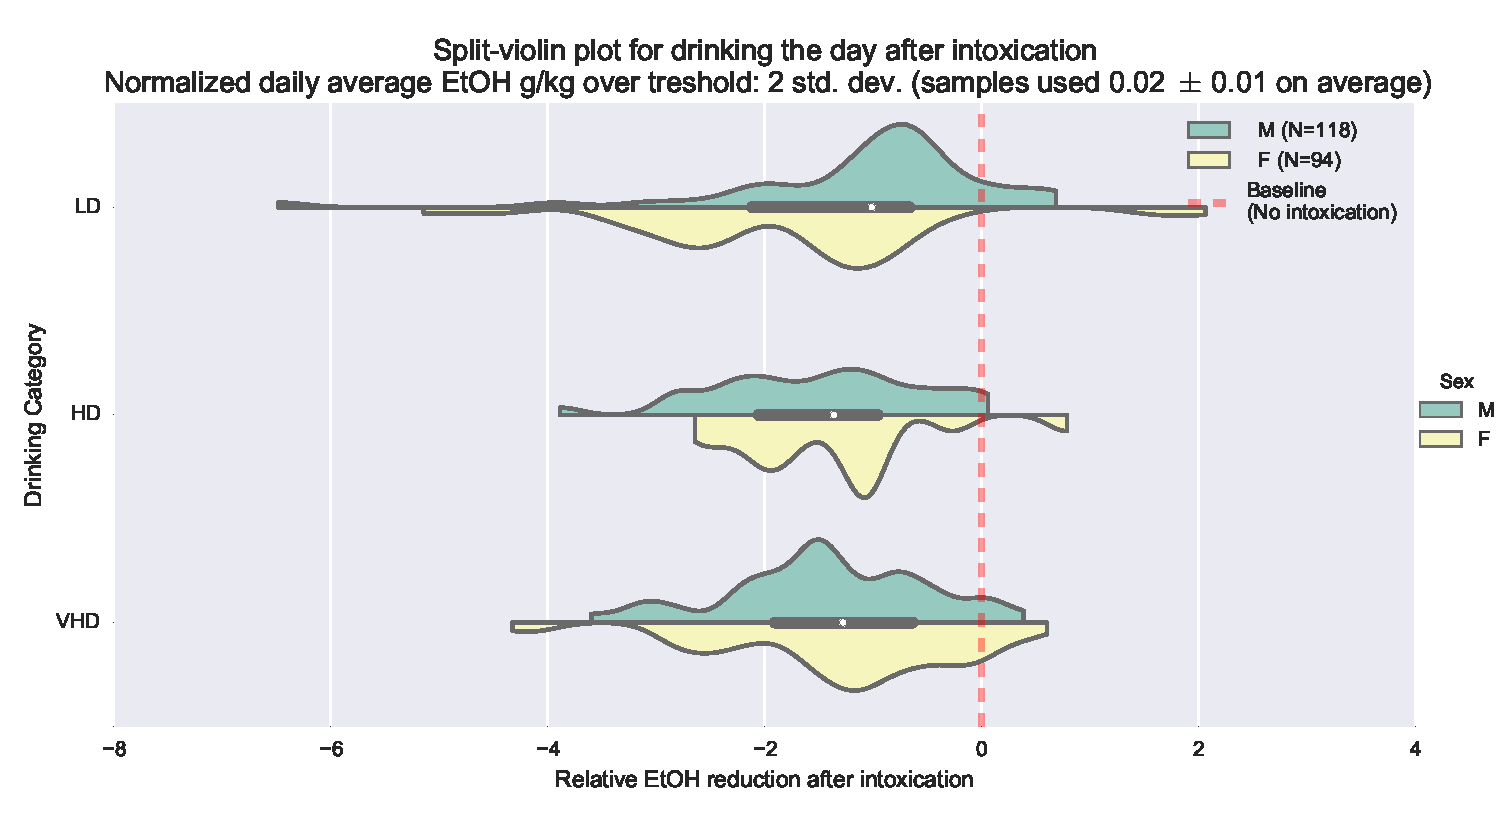
\includegraphics[width=\linewidth]{figures/intox_split-violin_mf.pdf}
		\caption{Split-violin plot for drinking the day after intoxication. Violin shows the details of reduction of drinking the day after intoxication (2\% of total drinking days), for each drinking category and for each gender.}
		\label{fig:intox-violin}	
	\end{figure}
	
	 
	
%	\begin{lstlisting}[language=Java]	
%	TM:
%	TM.releaseResources(TRID)	
%	\end{lstlisting}
\pagebreak	
\section{Predicting Future Drinkers \label{section:predicting-drinkers}}
	The following study demonstrates that data derived from the induction phase of the ethanol self-administration experiment has significant predictive power of whether or not an animal will go on to consume excessive alcohol in the future (during Open Access phase). Furthermore, we distinguish several factors tightly coupled with the probability of eventually being categorized as an heavy drinker. Early identification of risk factors in the NHP model lead to potential indicators in humans, resulting	in intervention and prevention.
	
	\subsection{Attributes' Predictive Power}
	\begin{figure}[ht]
		\centering
		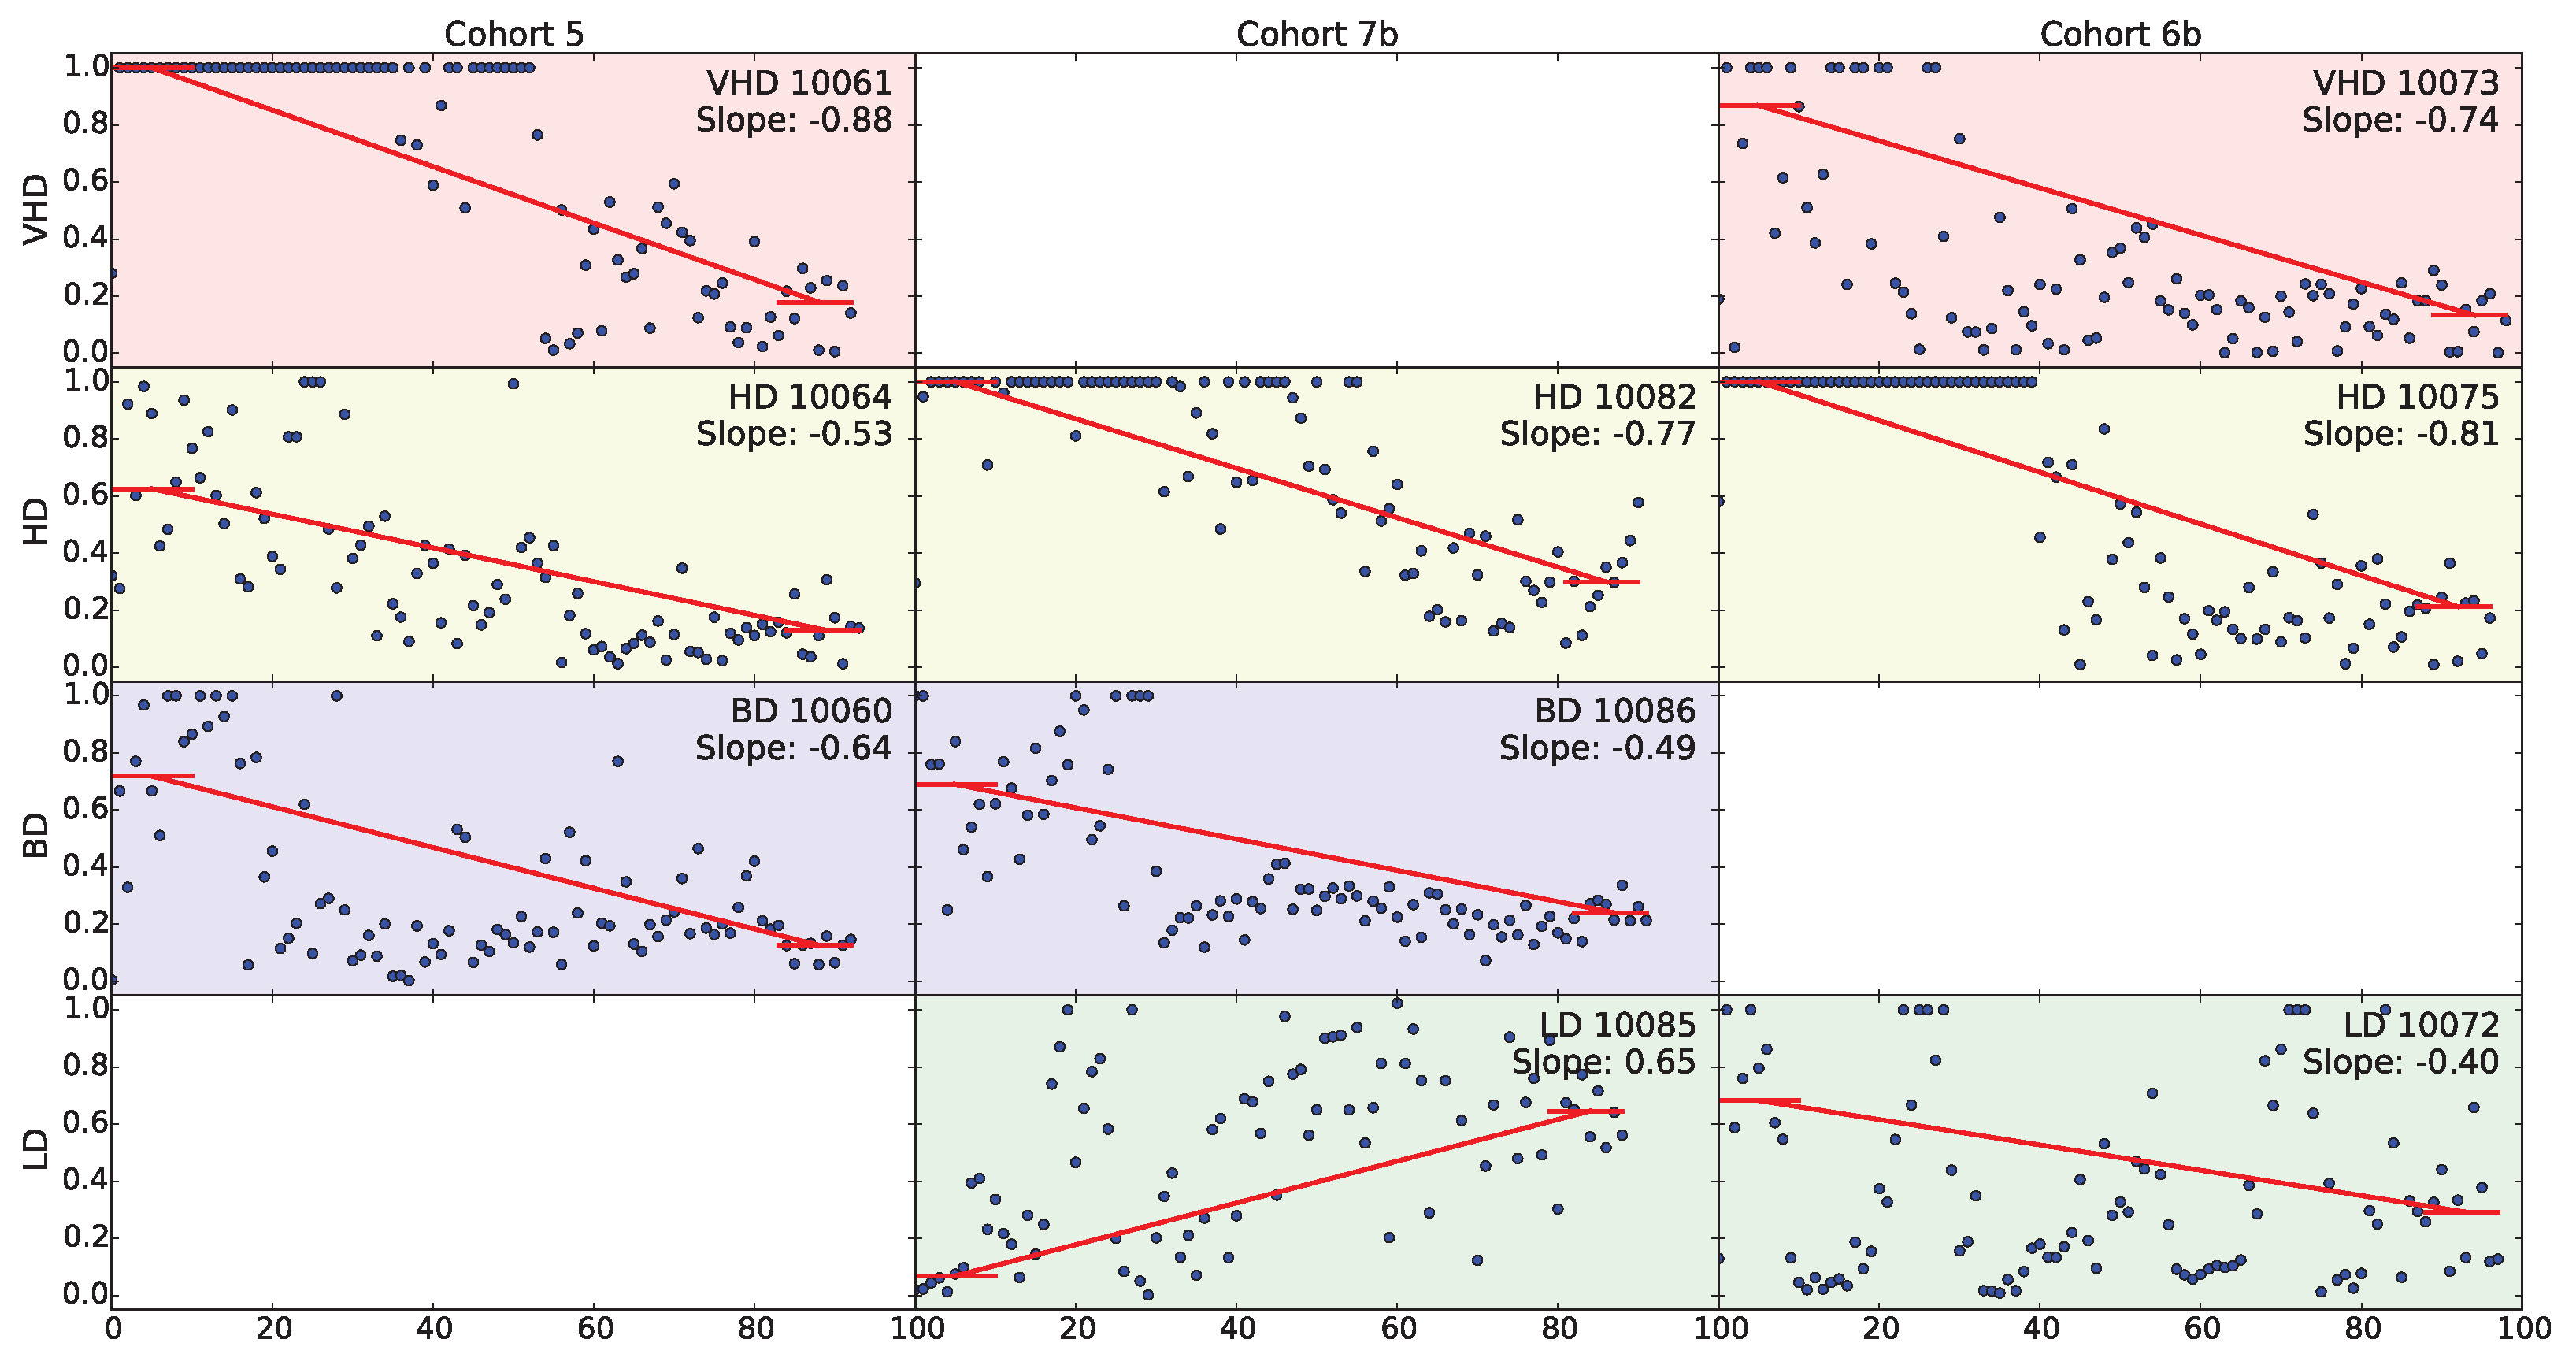
\includegraphics[width=\linewidth]{figures/attributes-predictive-power.pdf}
		\caption{Linear regression fit lines panels for each drinking category in three different cohorts illustrate persistent pattern indicating the predictive power of the attribute ``EtOH consumed during the first 10 minutes of the day, as a \% of day's total''.}
		\label{fig:attributes}	
	\end{figure}
	To demonstrate the predictive power of the attributes, consider Figure~\ref{fig:attributes}, which depicts the EtOH consumed during the first 10 minutes of the day, shown as a percent of the daily allotment. The plots are broken down by drinking categories and cohorts. From the figure we notice that the slope tends to be step negative for VHD and flattened step or even positive for LD. This difference indicates that the EtOH consumed during the first 10 minutes of the day is a potential prediction feature. 


	\subsection{Feature Generation}	
	Having over 20 raw and derived attributes we generated over 60 features in form of relative deltas as described in \cref{section:feature-generation}.
	\begin{figure}[ht]
		\centering
		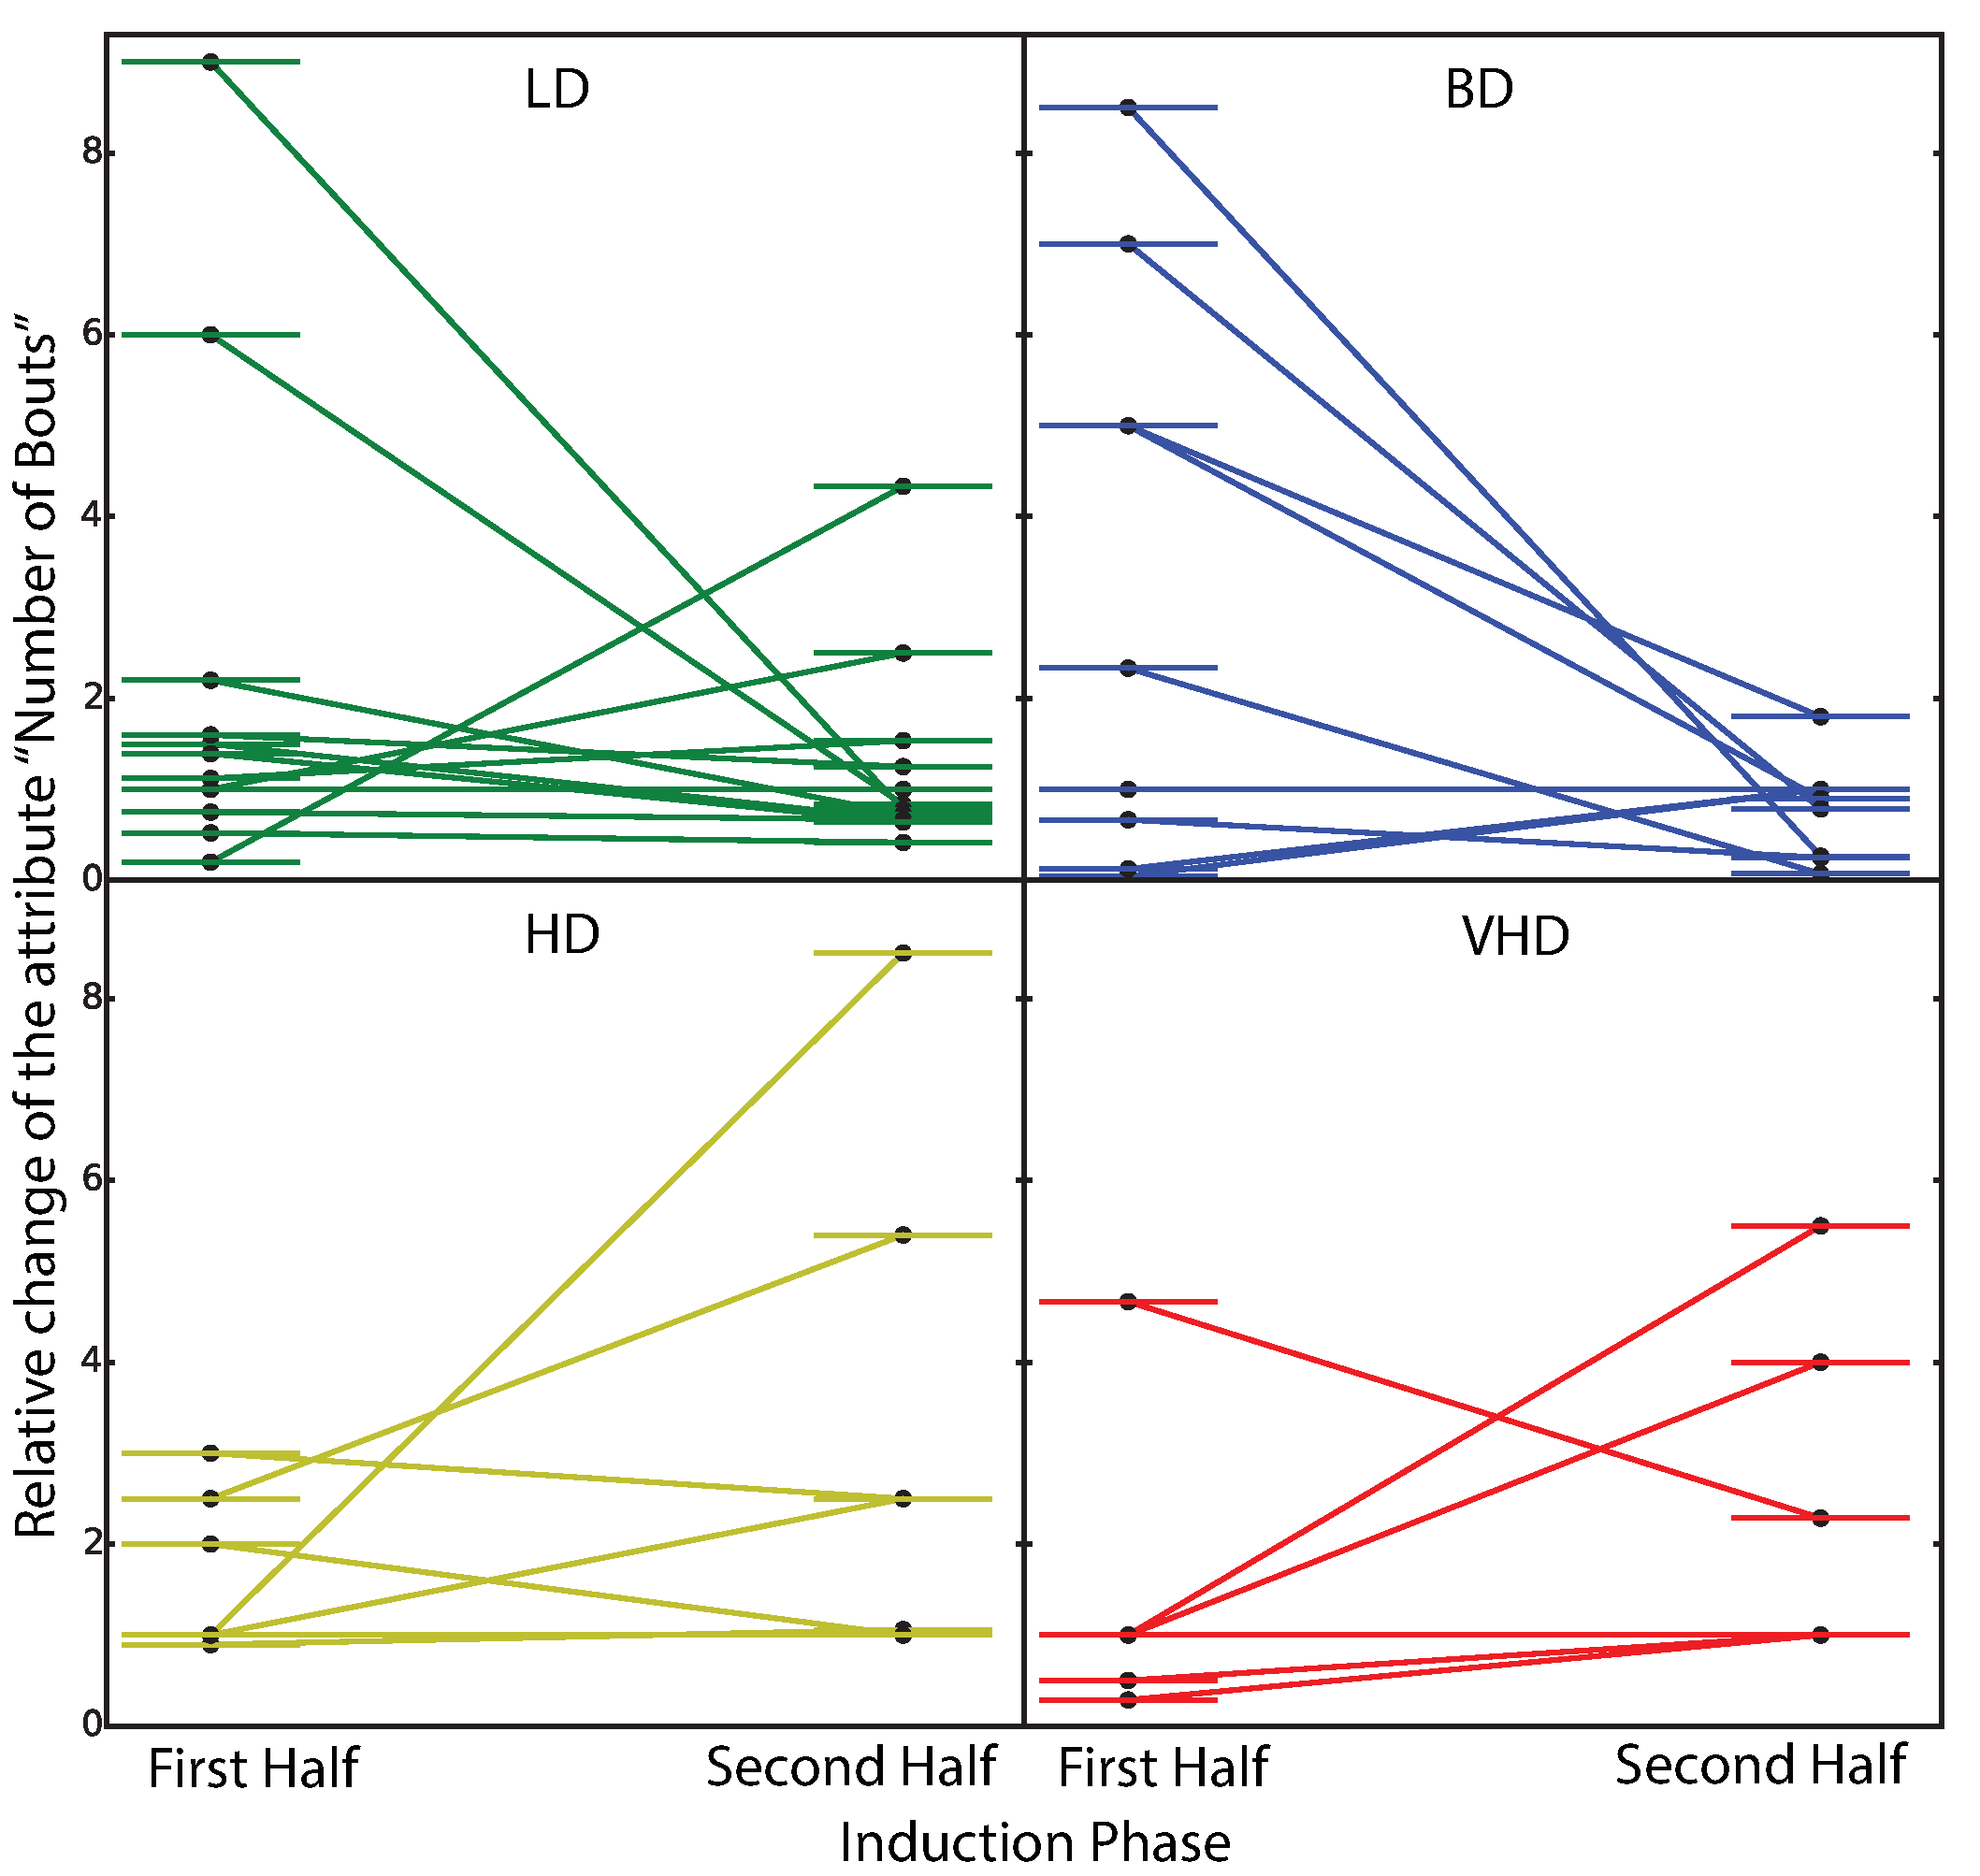
\includegraphics[width=0.8\linewidth]{figures/rel_change_num_bouts.pdf}
		\caption{Intra-cohort relative deltas panels for each drinking category illustrates persistent pattern in feature ''total number of EtOH bouts".}
		\label{fig:rel-change-bouts}	
	\end{figure}
	
	To illustrate the utility of relative deltas, Figure~\ref{fig:rel-change-bouts} displays the panel with relative deltas for the total number of EtOH bouts by a monkey during a 22-hour drinking session, divided into four subplots by drinking category. On the left of each plot, the figure indicates the relative change between the median values of phase one to phase two; on the right of each plot, the figure shows the relative change from phase two to phase three. The vertical axis represents the results from dividing the later median by the former. Low drinking animals, shown in the top row of the figure, generally decreased the total number of EtOH bouts on the later stage of the induction period (which could indicate either more aggressive bouts or less overall ethanol consumption), while high drinking animals generally increased by that same number. In this case, the calculation of relative deltas represents good predictors, or good features, because they describe the temporal process of drinking behavior adaptation. This is in-line with previous findings indicating that the third phase of induction, which is used to calculate relative deltas, is one of the most significant attributes in predicting drinking behavior \shortcite{grant2008drinking}.
	
	\subsection{Feature Filtering}
	Many features with small sample size lead to mathematically undetermined solutions. To filter the feature space we eliminated statistically non-significant features by performing significance tests ($\alpha=0.1$) and mutual information analysis. That leaves us with the most significant features shown in Figure~\ref{tab:feat-most-signif}, grouped by categories and ordered by p-value (decreasing top to the bottom). 
	
	A feature filtering step is used for selecting the best model. Later in this study we select a basis model and build on top of it. That novel model is developed using a feature selection technique, as described in \cref{section:feature-selection}.
	
	\begin{table}[h]
		\centering
		\caption{Feature space filtered by statistical significance.}
		\label{tab:feat-most-signif}
		\begin{tabular}{lll}
			\hline
			\abovespace\belowspace
			Feature & Phase & p-value\\
			\hline
			\multicolumn{3}{c}{Natural}\\
			\hline
			Age of intoxication & natur. & .004\\
			Age & natur. & .005\\
			Sex & natur. & .065\\
			\hline
			\multicolumn{3}{c}{Drinks}\\
			\hline
			Mean length for EtOH drinks & $\Delta_2$ & .003\\
			Mean volume for EtOH drinks & $\Delta_{total}$ & .014\\
			Median time between EtOH drinks & $\Delta_{2}$ & .036\\
			\hline
			\multicolumn{3}{c}{Bouts}\\
			\hline
			Total number EtOH bouts & $\Delta_{2}$ & .030\\
			Max bout volume as \% of total EtOH & $\Delta_{2}$ & .047\\
			Time to reach day's allotment & $\Delta_{2}$ & .097\\	
			\% EtOH during first 10 minutes & $\Delta_{1}$ & .080\\	
			Latency to first drink & $\Delta_{2}$ & .093\\
			Max bout length & $\Delta_{1}$ & .100\\			
			\hline
		\end{tabular}
	\end{table}

	\subsection{Model Selection}
	To select the basis model for the classification task we tested several models, see \cref{section:ml-models}. Acknowledging the noisy data with small sample size we tested each model with and without an applied bagging wrapper. Our hypothesis, regarding bootstrap aggregation, was that it should significantly improve the accuracy of Random Forests as suggested by \shortcite{breiman1996bagging}, but leave the Gradient Boosting without considerable changes since it natively incorporates its own special sampling technique. Ultimately, we could not draw hypothesis with regard to SVM. 
	
	\subsubsection{Support Vector Machines}
	We trained SVM models with various combination of parameters, as shown provided in Table~\ref{tab:svm-pars}. 
	
	\begin{table}[h]
		\centering
		\caption{Tested domain of settings for SVM classifier.}
		\label{tab:svm-pars}
		\begin{tabular}{lll}
			\hline
			\abovespace\belowspace
			Kernel	& Penalization Factor & Class Weights\\
			\hline
			Linear	& C = 1 & Yes\\
			Rbf (exponential) & C = 2 & No\\
			Polynomial & C = 3 &\\
			Sigmoid & C = 4 &\\		
			\hline
		\end{tabular}
	\end{table}
	
	Kernel could be thought as a similarity measure. Penalization factor sets the cost for the data that does not fit the current model; increasing C yields a more complex model (more feature are selected). Using class weights allow to counteract the problem of classes with unequal size. After repetitive experiments, model with the linear kernel and penalization factor C = 3 using sample weights proved to be the best option, having the mean accuracy, on average over multiple runs, equal 0.51 (SEM=.08). 
	
	\subsubsection{Random Forests}
	Random Forests (RF) are known to be very robust to the noise and to give good results while working fast.
	After repetitive experiments, we found the model with the following parameters to give the best accuracy: number of estimators=10, criterion=``gini", no max depth restriction, min samples split=2, min samples leaf=1, max features=0.4, bootstrap=True. This model yields a mean accuracy of .50 (SEM=.11), on average, which is not worse than SVM yet has greater variance. 
	
	\subsubsection{Gradient Boosting Classifier}
	A gradient Boosting (GB) classifier is an additive model in a forward stage-wise fashion; it allows for the optimization of arbitrary differentiable loss functions. In each stage, n-classes regression trees are fit on the negative gradient of the binomial or multinomial deviance loss function. Furthermore, it allows for sampling with the replacement with varying percentage of usage for number of features and number of examples used while training each individual tree. The best parameters for the model are: number of estimators = 200, max samples = 80$\%$, max features = sqrt, bootstrap = true. Thus, each of the 200 regressors trees had sampled, with replacement, set with size equals 80 $\%$ of examples, and, most importantly, with number of features equal square root of total number of available features. With that, GB yielded the mean accuracy of 56$\%$ (SEM=.1), on average. That is significantly better than both Random Forests and SVM yet variance kept in bounds. 
	
	\subsubsection{Bagging Wrapper}
	Since we have only 50 samples, and getting more is both costly and unethical, we tried to artificially sample (with replacements) more examples. Given arbitrary abundant feature sets we leave some of them behind in order to compensate for potentially meaningless features. That is exactly what Bagging Wrapper is meant to do with previous classifiers. Table~\ref{tab:ml-model-results} describes how bagging influences the classifiers and provides overall accuracy measures for each tested classifier along with the naive classifier described in \cref{section:performance-measure}. 
	
	\begin{table}[h]
		\centering
		\caption{Experimental accuracy results for different classifiers.}
		\label{tab:ml-model-results}
		\begin{tabular}{lll}
			\hline
			\abovespace\belowspace
			Classifier	& No Wrapper	& Bagging Wrapper \\
			\hline
			Naive & \multicolumn{2}{c}{0.32}\\
			SVM	 	& 0.51 (SEM=.08)	&	0.42 (SEM=.09)\\
			RF	&	0.50 (SEM=.11)	&  \textbf{0.61 (SEM=.07)}\\
			GB & 0.56 (SEM=.10)	& 0.57 (SEM=.10) \\	
			\hline
		\end{tabular}
	\end{table}
	
	Cohesive with our initial hypothesis, while Random Forests drastically improved its accuracy, Gradient Boosting result exhibit minimal change since it already incorporated some of the bagging technique and too extreme samples of bagging might have hurt the features gradients.
	
	SVM actually decreased its accuracy when used in conjunction with bagging. This might be explained by the fact that the regularization parameters for this model were fine tuned on the given dataset of 50 examples, thus sampling more of them destroyed the accurate settings of the model.
	
	To understand the difference in trade-off between the random forests and gradient boosting we could think of the fact that the better generalization property of ensemble approach is often explained using the classic bias-variance decomposition analysis. Specifically, previous studies pointed out that methods like bagging improve generalization by decreasing variance while methods similar to boosting achieve this by decreasing
	bias\footnote{In the article cited reader can find a visual representation of the mentioned differences.} \shortcite{yang2010review}.
		
	Given the above results, a random forests model with a bagging wrapper was chosen as basis model to perform two-step classification.	
	
	\subsection{Novelty Two-Step Classification Model}	
	The problem in our classification task is that given small sample size (50 animals) and uneven drinking class size distribution it is hard to train a good classifier. Thus we decided to perform classification in the two-steps. We first aggregated the four categories into two: ``LD and BD" and ``HD and VHD", essentially producing ``Heavy vs. Non-Heavy Drinkers". Then we used the basis RF model with bagging, but this time deploying forward selection strategy to rank the importance of each feature in order to reduce feature set dimensionality. Detailed description for feature selection procedure is provided in \cref{section:feature-selection}, but  essentially the process ranks the features by their impact on model performance. This process was a major computational bottleneck in building the classification model and took approximately 15 minutes each time. 
	
	During the first step, the classification accuracy for two groups reaches 82\%, and the best when using four features, as shown on the Figure~\ref{fig:forward-selection-combined}. There are three options on how to pick the features then. Initially, during each run of the feature selection procedure, we assigned the rankings to each feature, then we picked the top-4 most popular features according to the cumulative ranking. Another attempt was to rank features by the number of appearances in the top-4 list, simulating the essentialness of the features. Unexpectedly, both methods proved to be inferior to merely \textit{picking the top-4 features out of the best run}. That may be due to the fact, that feature selection process appends features \textit{based on their collaborative performance}, thus \textit{most popular features do not necessarily work well together}. 
	
	\begin{figure}[ht]
		\centering
		\includegraphics[width=\linewidth]{figures/feature-selection-heavy-non-eps-converted-to.pdf}
		\caption{Feature selection process for heavy vs. non-heavy drinkers.  The horizontal axis represents the number of features chosen based on contribution. The vertical axis shows the average accuracy of the drinking category classification. Base accuracy shows naive guess.}
		\label{fig:forward-selection-combined}
	\end{figure}
	
	On the second step, aggregated categories were subsequently reclassified into their individual inherent categories: non-heavy drinkers into LD and BD, heavy drinkers into HD and VHD. The feature selection procedure produced the set of features that results in the best average accuracy. Table~\ref{tab:selected-features} provides a summary of selected features during each step and the average accuracy.
	
	\begin{table}[htb]
	\centering
	\caption{Set of features chosen by \textit{Forward Selection} algorithm for two-step model classification. For each of the three classification tasks the sets of selected features are different which may relate to the different nature of behavioral characteristics between difference drinking groups.}
	\label{tab:selected-features}
	\begin{tabular}{ll}
	\hline
	\abovespace\belowspace
	\toprule Feature & Phase  \\ \midrule		
	\multicolumn{2}{c}{\textit{Heavy vs Non-Heavy Drinkers (accuracy=0.82)}} \\
	Number of EtOH bouts & $\Delta_2$ \\
	Mean length for EtOH drinks &  $\Delta_1$\\
	Mean volume for EtOH drinks & $\Delta_1$\\
	Age & \textit{fixed}\\ 
	
	\midrule
	\multicolumn{2}{c}{\textit{Low vs Binge Drinkers (accuracy=0.91)}} \\
	Mean length for EtOH drinks &  $\Delta_2$\\
	Latency to the first drink & $\Delta_{total}$\\
	
	\midrule
	\multicolumn{2}{c}{\textit{Heavy vs Very Heavy Drinkers (accuracy=0.89)}} \\
	\% of days EtOH consumed in first bout &  $\Delta_{total}$\\
	EtOH during first 10 minutes of the day & $\Delta_{total}$ \\ 	
	\bottomrule
	\end{tabular}
	\end{table}
	
	For the heavy vs. non-heavy drinkers classification we can achieve a 82\% accuracy rate with four features: total number of EtOH bouts, mean length and volume of EtOH drinks, and age. Distinguishing between subgroups appears to be even more accurate, however that is due to  fact that the class size distribution is more skewed within the subgroups. 
	
	Observing the absence of common features between classification of two sub-groups indicates that the differentiation between HD and VHD is markedly distinct from the differentiation between LD and BD. This may relate to the different nature of behavioral characteristics between difference drinking groups. Notably, for HD and VHD, both features are associated with the drinking within the first minutes of the day, while for distinguishing heavy and non-heavy drinkers the mean values describing drinks are predicative.


	\subsection{Model Validation}
	To validate the model we calculated two-step composite average accuracy and the by-cohort accuracy using the evaluation tools described in \cref{section:accuracy-evaluation} and \cref{section:performance-measure}.
	
	\subsubsection{Two-Step Composite Average Accuracy} Total, or composite, accuracy is calculated for the entire model by determining category distribution and the accuracy rates for both the first and second steps. The prior probability of a sample being in the group ``LD and BD" is 52\%, while the prior probability (or likelihood) of being in the group ``HD and VHD" is 48\%. Accordingly, the probability-adjusted accuracy of being correctly classified within the Heavy and Non-Heavy groups is 82\%. The first step accuracy of 82\% and formula~\ref{eq:composite-accuracy} is used to composite average accuracy. \textit{P} denotes the prior probability (or likelihood) in [0..1] format; \textit{A} denotes accuracy: 
	\begin{equation}
	\begin{split}
	A_{comp.} &= A_{1^{st}step}*(P(non-heavy)*A_{LD vs. BD} + P(heavy)*A_{HD vs. VHD})\\
			&= 0.82*(0.48 * 0.89 + 0.52*0.91) = 0.74
	\end{split}
	\label{eq:composite-accuracy}
	\end{equation}
	
	To measure the improvement of the composite average accuracy of 74\% we compare it to the base case accuracy. To calculate the base case for two-step classification by choosing the most likely categories during both steps. In the first step, the most likely group is ``LD and BD" with a 52\% probability of being correct. In the second step, the most likely category is LD with a 62\% probability of being correct. Thus, the overall accuracy for a two-step naive classifier is 32\%. Our classification strategy represents approximately a 2.5 fold performance improvement over a naive probabilistic way of predicting the correct result. 
	
	
	\subsubsection{Cohort Accuracy} While animals come from different cohorts, their common experimental protocol backgrounds enable an evaluation of common behavioral features that may help to predict future drinking associated with AUDs. Examination in a cohort-centric manner, however, reveals information about cohort specific behavior. 
	
	To calculate the accuracy by cohort, instead of random folds as in cross-validation we used cohorts division as natural folds. For each such fold (cohort) we trained the model on all the other examples outside of the fold and then tested on the chosen fold\footnote{Importantly, the cohort id information was unavailable for the model which otherwise would have made the task much simpler due to the skewed DC distribution within cohorts.}. Table~\ref{tab:by-cohort-heavy-non} provides the results of the first step classification accuracy by cohort. Such table were also create for two classification tasks of the second step and could be found in Appendix A, Table~\ref{tab:by-cohort_ld_bd} and \ref{tab:by-cohort_hd_vhd}.
	
	\begin{table}[h]
	%---HEAVY VS NON-HEAVY
	\centering
	\caption{First step (heavy vs non-heavy) classification accuracy using cross-validation with the cohorts as natural folds.}
	\label{tab:by-cohort-heavy-non}
	\begin{subfigure}{0.3\linewidth}  \centering	
	\begin{tabular}{ll}	
		\hline
		\abovespace\belowspace
		\toprule Cohort & Accuracy\\ \midrule
		Rhesus 4 &  0.7\\
		Rhesus 5 & 0.625\\
		Rhesus 6a &  0.83\\
		Rhesus 6b & 1.0\\
		Rhesus 7a & 0.5\\
		Rhesus 7b &  0.8\\
		Rhesus 10 & 0.875\\ \bottomrule
	\end{tabular}
	\caption{Accuracy \label{table:by-cohort-accuracy-twocases}}		
	\end{subfigure}
	\begin{subfigure}{0.3\linewidth}\centering
	\begin{tabular}{ccc}
		\toprule  & \multicolumn{2}{c}{Predicted DC}\\ 
		\cmidrule(r){2-3}
		DC & Heavy & Not \\ \midrule
		Heavy & 5 & 21 \\
		Not & 16 & 8\\ \bottomrule
	\end{tabular}
	\caption{Confusion Matrix \label{table:by-cohort-cm-twocases}}		
	\end{subfigure}	
	\begin{subfigure}{\linewidth}\centering
		\begin{tabular}{lllll}
			\toprule DC &  precision  & recall & f1-score  & support\\	\midrule
			Heavy    &   0.72   &   0.81   &   0.76    &    26 \\
			Non-heavy     &  0.76   &   0.67   &   0.71    &    24\\
			Avg / Total    &   0.74   &   0.74   &   0.74   &  50\\ \bottomrule
		\end{tabular}
		\caption{Per class recall, presicion, f-measure and support\label{table:by-cohort-cm-details-twocases}}	
	\end{subfigure}	
	\end{table}
	
	While our classifier performs relatively well, since cohort sizes are extremely small it is difficult to use intra-cohort predictions as the basis for inter-cohort hypotheses development or to draw conclusions about the population in total. 


	\subsection{Partial Dependencies}
	The downside of the RF classifier is that it is hard to infer the features influence onto target variable. In our case we are interested to see how each feature, or combination of features, affects the likelihood of the later drinking category classification to the animal. We use partial dependency plots (PDP) to facilitate the visual understanding of the dependence between the likelihood of becoming very heavy drinker (VHD) and a set of target features, marginalizing over the values of all other features. 	
	
	\begin{figure}[ht]
		\centering
		\includegraphics[width=0.8\linewidth]{figures/pdp5-eps-converted-to.pdf}
		\caption{Partial dependence plots (PDP) illustrate the dependence between the two target features (maximum bout length and mean length of EtOH drinks) and the likelihood of becoming VHD (top row) or LD (bottom row).}
		\label{fig:pdp5}
	\end{figure}
	
	Figure~\ref{fig:pdp5} provides two PDP plots. Top row describes the dependence between two target features and the likelihood of becoming VHD. Feature relative change of the tendency (mean or median) is normalized by standard deviation and adjusted by animal's weight and plotted on the x-axis. Feature values represent fold changes: a value of 2 on x-axis means that animal increased the value of this attribute two-fold during the induction, while value 0.5 means decreasing two-fold. 
%	Vertical bars on the x-axis represent a sample used for the line approximation. 
	
	First, consider the feature ``Max bout length". There is a linear relationship that implies animals that increased their maximum bouts’ length during the induction are very likely to become VHD later on. That may indicate that, in general, future VHD animals prefer alcohol and start to enjoy it and prolong their maximum bouts in time. However, there are several VHDs that do not fit that pattern, and while they increased their max bouts' length significantly they were less likely to become VHD. This constitutes either a factor unaccounted for or the erroneous classification method for that specific animals. Second, consider the feature ``Mean length of EtOH drinks".  Animals that either increased or decreased the average length of their alcohol drinks were less likely to become VHD, while those who did not change that preference much were. It is not clear why is that, however PDP for the likelihood of LD creates a potential insight.
	
	Contrast the previous results with the bottom row, which describes the dependence between the same two target features and the likelihood of becoming LD. The more animals increased their max bouts' length, relatively to the initial max bout length, the less likely they were later classified as LD. That may indicate that low drinking animals do not create a strong preference for alcohol and prefer to gulp it (since they have learned that they have to), rather than sip and enjoy it. On the other hand, there is a linear relationship between the increase in the mean length of alcohol drinks and the chances of later being classified as LD. That may indicate that despite low drinking animals do not like to have a long alcohol bouts, they do not like to do short and fast ``shots" either. 
	
	The fact that partial dependencies for opposing drinking categories are overall consistent with each other verifies the validity of the method. Figures~\ref{fig:VHD_gradients} and \ref{fig:LD_gradients} in appendix B provide eight additional PDPs of the likelihood of being classified as VHD or LD on alternative set of target features.

	
